\documentclass{article}
\usepackage[utf8]{inputenc}


\newcommand{\lsp}{\vspace{3mm}}
\newcounter{remark}[section]
%\usepackage[dvips]{color}

%\usepackage[top=26mm, bottom=26mm, left=32mm, right=32mm]{geometry}



%&LaTeX

%%% This document contains macros that will be used throughout
%%% It is very neatly organized.


%%%%% Packages

%\usepackage[notcite]{showkeys}

\usepackage{amsmath}
\usepackage{amssymb}
\usepackage{bm}
\usepackage{mathrsfs}
\usepackage[dvips]{graphicx}
%\usepackage{stmaryrd}
%\usepackage{wasysym}

\usepackage{color}

\usepackage{url}
% \usepackage{citesort}

%\usepackage{supertabular}


%%% Algorithm package

%\usepackage{alg}

%\renewcommand{\thealgorithmfloat}{\thesection.\arabic{algorithmfloat}}

%% Commands dealing with alg.sty
\makeatletter
%\def\algspacing{\alg@unmargin}
\makeatother

\newcommand{\algfor}[1]{\textbf{for} #1\\\algbegin}


%%% Theorem setup

\newtheorem{fact}{Fact}

%\theoremstyle{plain}

%\newtheorem{bigthm}{Theorem}
%\renewcommand{\thebigthm}{\Alph{bigthm}}    % Number with A, B, C, etc.
%\newtheorem{thm}{Theorem}
%\newtheorem{cor}[thm]{Corollary}
%\newtheorem{lemma}[thm]{Lemma}
%\newtheorem{prop}[thm]{Proposition}

%\theoremstyle{definition}
%\newtheorem{defn}[thm]{Definition}

%\newtheorem{algorithm}[thm]{Algorithm}

%\theoremstyle{remark}
%\newtheorem{remark}[theorem]{Remark}

%\newtheorem*{notation}{Notation}

%\numberwithin{equation}{section}
%\numberwithin{thm}{section}

%\numberwithin{figure}{chapter}
%\numberwithin{table}{chapter}


%%% Typesetting

\DeclareMathAlphabet{\mathsfsl}{OT1}{cmss}{m}{sl}


%%% Other font changes

\newcommand{\lang}{\textit}
\newcommand{\titl}{\textsl}
\newcommand{\term}{\emph}

%\newcommand{\algname}{\textsc}

\newcommand{\cnst}[1]{\mathrm{#1}}


%%% New environments

\newenvironment{inputs}%
    {\makebox{\phantom{}} \\ %
        \textsc{Input:}\begin{itemize}}%
    {\end{itemize}}

\newenvironment{outputs}%
    {\textsc{Output:}\begin{itemize}}%
    {\end{itemize}}

\newenvironment{procedure}%
    {\textsc{Procedure:}\begin{enumerate}}%
    {\end{enumerate}}


%%% Old symbols with new names

\newcommand{\oldphi}{\phi}
\renewcommand{\phi}{\varphi}

\newcommand{\eps}{\varepsilon}


%%% New symbols

\newcommand{\defby}{\overset{\mathrm{\scriptscriptstyle{def}}}{=}}
\newcommand{\half}{\tfrac{1}{2}}
\newcommand{\third}{\tfrac{1}{3}}



%%% Constants

\newcommand{\econst}{\mathrm{e}}
\newcommand{\iunit}{\mathrm{i}}

\newcommand{\onevct}{\mathbf{e}}
\newcommand{\zerovct}{\vct{0}}

%\newcommand{\Id}{\mathsf{I}}
%\newcommand{\onemtx}{\mathsf{1}}
%\newcommand{\zeromtx}{\mathsf{0}}

\newcommand{\Id}{\mathbf{I}}
\newcommand{\onemtx}{\bm{1}}
\newcommand{\zeromtx}{\bm{0}}


%%% Sets

\newcommand{\coll}[1]{\mathscr{#1}}

\newcommand{\Sspace}[1]{\mathbb{S}^{#1}}

\newcommand{\Rplus}{\mathbb{R}_{+}}
\newcommand{\Rspace}[1]{\mathbb{R}^{#1}}
\newcommand{\Cspace}[1]{\mathbb{C}^{#1}}

\newcommand{\RPspace}[1]{\mathbb{P}^{#1}(\mathbb{R})}
\newcommand{\CPspace}[1]{\mathbb{P}^{#1}(\mathbb{C})}
\newcommand{\FPspace}[1]{\mathbb{P}^{#1}(\mathbb{F})}

\newcommand{\RGspace}[2]{\mathbb{G}( {#1}, \Rspace{#2} )}
\newcommand{\CGspace}[2]{\mathbb{G}( {#1}, \Cspace{#2} )}
\newcommand{\FGspace}[2]{\mathbb{G}( {#1}, \mathbb{F}^{#2} )}

\newcommand{\RR}{$\Rspace{}$}
\newcommand{\CC}{$\Cspace{}$}

\newcommand{\Mset}[1]{\mathbb{M}_{#1}}

\newcommand{\oneton}[1]{\left\llbracket {#1} \right\rrbracket}


%%% Real and complex analysis

\newcommand{\abs}[1]{\left\vert {#1} \right\vert}
\newcommand{\abssq}[1]{{\abs{#1}}^2}

\newcommand{\sgn}[1]{\operatorname{sgn}{#1}}
\newcommand{\real}{\operatorname{Re}}
\newcommand{\imag}{\operatorname{Im}}

\newcommand{\diff}[1]{\mathrm{d}{#1}}
\newcommand{\idiff}[1]{\, \diff{#1}}

%\newcommand{\grad}{\nabla}
\newcommand{\subdiff}{\partial}

\newcommand{\argmin}{\operatorname*{arg\; min}}
\newcommand{\argmax}{\operatorname*{arg\; max}}

\newcommand{\psdge}{\succcurlyeq}
\newcommand{\psdle}{\preccurlyeq}

%%% Probability

\newcommand{\Probe}[1]{\mathbb{P}\left({#1}\right)}
\newcommand{\Prob}[1]{\mathbb{P}\left\{ {#1} \right\}}
\newcommand{\Expect}{\operatorname{\mathbb{E}}}
\newcommand{\Var}{\operatorname{Var}}

\newcommand{\normal}{\textsc{normal}}
\newcommand{\erf}{\operatorname{erf}}



%%% Vector and matrix operators

\newcommand{\vct}[1]{\bm{#1}}
\newcommand{\mtx}[1]{\bm{#1}}
%\newcommand{\mtx}[1]{\mathsf{#1}}
%\newcommand{\mtx}[1]{\mathsfsl{#1}}


\newcommand{\transp}{\mathrm{T}}
\newcommand{\adj}{*}
\newcommand{\psinv}{\dagger}

\newcommand{\lspan}[1]{\operatorname{span}{#1}}

\newcommand{\range}{\operatorname{range}}
\newcommand{\colspan}{\operatorname{colspan}}

%\newcommand{\rank}{\operatorname{rank}}
\newcommand{\strank}{\operatorname{st.rank}}

%\newcommand{\diag}{\operatorname{diag}}
\newcommand{\trace}{\operatorname{trace}}

%\newcommand{\supp}[1]{\operatorname{supp}(#1)}

\newcommand{\smax}{\sigma_{\max}}
\newcommand{\smin}{\sigma_{\min}}


%%% Mensuration: inner products and norms

\newcommand{\ip}[2]{\left\langle {#1},\ {#2} \right\rangle}
\newcommand{\absip}[2]{\abs{\ip{#1}{#2}}}
\newcommand{\abssqip}[2]{\abssq{\ip{#1}{#2}}}
\newcommand{\tworealip}[2]{2 \, \real{\ip{#1}{#2}}}

\newcommand{\norm}[1]{\left\Vert {#1} \right\Vert}
\newcommand{\normsq}[1]{\norm{#1}^2}

    % Fixed-size inner products and norms are useful sometimes

\newcommand{\smip}[2]{\bigl\langle {#1}, \ {#2} \bigr\rangle}
\newcommand{\smabsip}[2]{\bigl\vert \smip{#1}{#2} \bigr\vert}
\newcommand{\smnorm}[2]{{\bigl\Vert {#2} \bigr\Vert}_{#1}}

\newcommand{\enorm}[1]{\norm{#1}_2}
\newcommand{\enormsq}[1]{\enorm{#1}^2}

\newcommand{\fnorm}[1]{\norm{#1}_{\mathrm{F}}}
\newcommand{\fnormsq}[1]{\fnorm{#1}^2}

\newcommand{\pnorm}[2]{\norm{#2}_{#1}}
\newcommand{\infnorm}[1]{\norm{#1}_{\infty}}

\newcommand{\iinorm}[1]{\pnorm{\infty,\infty}{#1}}

\newcommand{\rxnorm}[1]{\pnorm{\mathrm{rx}}{#1}}

\newcommand{\dist}{\operatorname{dist}}

\newcommand{\triplenorm}[1]{\left\vert\!\left\vert\!\left\vert {#1} \right\vert\!\right\vert\!\right\vert}

\newcommand{\smtriplenorm}[1]{\big\vert\!\big\vert\!\big\vert {#1} \big\vert\!\big\vert\!\big\vert}

%%% Unusual operators

\newcommand{\cover}{\operatorname{cover}}
\newcommand{\pack}{\operatorname{pack}}
\newcommand{\maxcor}{\operatorname{maxcor}}
\newcommand{\ERC}{\operatorname{ERC}}
\newcommand{\quant}{\operatorname{quant}}
\newcommand{\conv}{\operatorname{conv}}
\newcommand{\spark}{\operatorname{spark}}

%%% Problem Names

\newcommand{\exactprob}{\textsc{(exact)}}
\newcommand{\rexact}{\textsc{(r-exact)}}
\newcommand{\errorprob}{\textsc{(error)}}
\newcommand{\rerror}{\textsc{(r-error)}}
\newcommand{\sparseprob}{\textsc{(sparse)}}
\newcommand{\subsetprob}{\textsc{(subset)}}
\newcommand{\rsubset}{\textsc{(r-subset)}}

\newcommand{\lonepen}{\textsc{($\ell_1$-penalty)}}
\newcommand{\loneerr}{\textsc{($\ell_1$-error)}}


%%% Things that get typed a lot

\newcommand{\Dict}{\coll{D}}

\newcommand{\opt}{\mathrm{opt}}
\newcommand{\bad}{\mathrm{bad}}
\newcommand{\err}{\mathrm{err}}
\newcommand{\alt}{\mathrm{alt}}
\newcommand{\good}{\mathrm{good}}

\newcommand{\subjto}{\quad\text{subject to}\quad}
\newcommand{\etal}{et al.\ }

\newcommand{\cost}[2]{\operatorname{cost}_{#1}(#2)}

\newcommand{\TF}{\mathrm{TF}}

\newcommand{\chord}{\mathrm{chord}}
\newcommand{\proj}{\mathrm{spec}}
\newcommand{\fs}{\mathrm{FS}}

\newcommand{\bigO}{\mathrm{O}}


%%% Constants, vectors and matrices with names

\newcommand{\atom}{\vct{\phi}}
\newcommand{\Fee}{\mtx{\Phi}}

\newcommand{\Lamopt}{\Lambda_{\opt}}

\newcommand{\astar}{\vct{a}_{\star}}
\newcommand{\aLam}{\vct{a}_{\Lambda}}
\newcommand{\aopt}{\vct{a}_{\opt}}

\newcommand{\Astar}{\mtx{A}_{\star}}
\newcommand{\ALam}{\mtx{A}_{\Lambda}}
\newcommand{\Aopt}{\mtx{A}_{\opt}}

\newcommand{\cLam}{\vct{c}_{\Lambda}}
\newcommand{\copt}{\vct{c}_{\opt}}

\newcommand{\CLam}{\mtx{C}_{\Lambda}}
\newcommand{\Copt}{\mtx{C}_{\opt}}

\newcommand{\bstar}{\vct{b}_{\star}}
\newcommand{\bLam}{\vct{b}_{\Lambda}}
\newcommand{\bbad}{\vct{b}_{\bad}}
\newcommand{\balt}{\vct{b}_{\alt}}
\newcommand{\bopt}{\vct{c}_{\opt}}

\newcommand{\Bstar}{\mtx{B}_{\star}}
\newcommand{\BLam}{\mtx{B}_{\Lambda}}
\newcommand{\Bopt}{\mtx{B}_{\opt}}
\newcommand{\Balt}{\mtx{B}_{\alt}}

\newcommand{\Ropt}{\mtx{R}_{\opt}}


\newcommand{\gamstar}{\gamma_{\star}}

\newcommand{\PhiLam}{\mtx{\Phi}_{\Lambda}}
\newcommand{\Phiopt}{\mtx{\Phi}_{\opt}}
\newcommand{\Phialt}{\mtx{\Phi}_{\alt}}
\newcommand{\Psiopt}{\mtx{\Psi}}
\newcommand{\PsiLam}{\mtx{\Psi}_{\Lambda}}


\newcommand{\Popt}{{\mtx{P}_{\opt}}}
\newcommand{\PLam}{{\mtx{P}_{\Lambda}}}

\newcommand{\GLam}{{\mtx{G}_{\Lambda}}}

\newcommand{\rhoerr}{\rho_{\err}}
\newcommand{\rhoopt}{\rho_{\opt}}

\newcommand{\success}{\mathrm{succ}}
\newcommand{\failure}{\mathrm{fail}}

\newcommand{\restrict}[1]{\vert_{#1}}


\newcommand{\anum}[1]{{\footnotesize{#1}\quad}}

%%%%% Stupid LaTeX tricks

\newcommand{\forcetall}{\phantom{\frac{1}{\frac{1}{1}}}}

\input{algorithm_labels.aux}

\newtheorem{remark}{Remark}
\newtheorem{theorem}{Theorem}

\title{Reading Course: Randomized Methods for Low-Rank Approximation}
\author{Farnaz IRANI}
\date{March 2018}

\begin{document}

\maketitle

\section{Introduction}
This is a reading course on the article \textit{Finding Structure with Randomness: Probabilistic Algorithms for Constructing Approximate Matrix Decompositions}, by N.~Halko, P.~G.~Martinsson, and J.~A.~Tropp.
We will explain some important results from this article, with focus on randomized methods for solving the low-rank approximation problem. This work is supervised by Prof.~Dr.~Bart, University of Geneva.


%\pgnotate{After ``constant'' maybe we should squeeze in a comment that
%this can mean as few as ``one''?}

% The recent development of randomized techniques for approximating
% numerically rank-deficient matrices is rapidly transforming
% numerical linear algebra. To illustrate this development, the
% present paper describes and analyzes a class of techniques for
% solving variations of a basic model problem: Given an $m\times n$
% matrix $\mtx{A}$ and an integer $k < \min\{m,n\}$, compute an
% $m\times k$ matrix $\mtx{B}$ and a $k\times n$ matrix $\mtx{C}$ such
% that $\norm{\mtx{A} - \mtx{B}\mtx{C}} \approx \min\{\norm{\mtx{A} -
% \mtx{A}_{(k)}}\,\colon\, \mtx{A}_{(k)}\mbox{ has rank }k\}$.
% Variations discussed include the imposition of conditions on the
% factors; for instance, the problem of computing an approximate
% Singular Value Decomposition, or an approximate (rank-revealing) QR
% factorization. Randomized techniques have proven highly effective at
% solving such approximation problems in a range of different
% environments, for instance: (1) For a general dense matrix
% $\mtx{A}$, accurate and stable randomized techniques require
% $O(mn\log(k))$ operations, as opposed to the $O(mnk)$ operations
% required by classical techniques. (2) For sparse matrices, and other
% matrices that can rapidly be applied to vectors, randomized
% techniques match the number of floating point operations required by
% state-of-the-art classical techniques such as Arnoldi or Lanczos,
% but are more robust, and allow much more flexibility in organizing
% the computation, allowing multi-core architectures to be exploited
% fully. (3) For very large matrices that do not fit in fast memory,
% randomized methods allow approximate factorizations to be computed
% out-of-core with as few as a single pass over the data.



\section{Low-Rank Approximation}
\label{sec:low}

Low-rank matrix approximations, such as the truncated singular value
decomposition and the rank-revealing QR decomposition, play a central
role in data analysis and scientific computing. Randomization offers a
powerful tool for performing low-rank matrix approximation.
These
techniques exploit modern computational architectures
more fully than classical methods and open the possibility of
dealing with truly massive data sets.


These methods
use random sampling
to identify a subspace that captures most of the action
of a matrix. The input matrix is then compressed---either explicitly
or implicitly---to this subspace, and the reduced matrix is
manipulated deterministically to obtain the desired low-rank
factorization.

The standard matrix decompositions includes the pivoted QR
factorization, the eigenvalue decomposition, and the singular value
decomposition (SVD), all of which expose the (numerical) range of a
matrix. Truncated versions of these factorizations are often used to
express a \emph{low-rank approximation} of a given matrix:
\begin{equation}
\label{eq:lowrank}
\begin{array}{ccccccccccc}
\mtx{A} &\approx& \mtx{B} & \mtx{C},\\
m\times n && m \times k & k\times n.
\end{array}
\end{equation}
The inner dimension $k$ is sometimes called the \emph{numerical rank} of the matrix.
When the numerical rank is much smaller than either dimension $m$ or $n$,
a factorization such as \eqref{eq:lowrank} allows the matrix to be stored
inexpensively and to be multiplied rapidly with vectors or other matrices.
The factorizations can also be used for data interpretation or to
solve computational problems, such as least squares.

Matrices with low numerical rank appear in a wide variety of scientific
applications:

%\notate{Steal references from other papers.  Compress this material.}

\begin{itemize}
\item   A basic method in statistics and data mining is to compute the
directions of maximal variance in vector-valued data by performing
\emph{principal component analysis} (PCA) on the data matrix.

%~\cite[Sec.~3.8]{DHS01:Pattern-Recognition},.
%This technique is ubiquitous in genomics, analysis of financial data, etc.

\item   Another standard technique in data analysis is to perform
low-dimensional embedding of data under the assumption that there
are fewer degrees of freedom than the ambient dimension would suggest.
In many cases, the method reduces to computing a partial SVD of a matrix
derived from the data.  %See~\cite[\S\S14.8--14.9]{HTF08:Elements-Statistical}
%or \cite{coifman_PNAS_diffusionmaps}.
This approach has been applied to study the link structure of the
World Wide Web and to compress and classify large
collections of images.
%This approach has been applied to study the link structure of the


\item The problem of estimating parameters from measured data via
least-squares fitting often leads to very large systems of linear
equations that are close to linearly dependent. Effective techniques
for factoring the coefficient matrix lead to efficient techniques
for solving the least-squares problem.

\item   Many fast numerical algorithms for solving PDEs and for rapidly evaluating
potential fields such as the fast multipole method~\cite{rokhlin1997}
and $\mathcal{H}$-matrices~\cite{hackbusch2003}, rely on low-rank approximations of
continuum operators.

\item Models of multiscale physical phenomena often involve PDEs with rapidly
oscillating coefficients. Techniques for  \emph{model reduction}
or \emph{coarse graining} in such environments are often based %(directly or indirectly)
on the observation that the linear transform that maps the input data to the requested output
data %(such as an average deflection, or an average porosity)
can be approximated by an operator of low rank.
\end{itemize}


The task of computing a low-rank approximation to a given matrix
can be split naturally into two computational stages. The first is
to construct a low-dimensional subspace that captures the action
of the matrix. The second is to restrict the matrix to the subspace
and then compute a standard factorization (QR, SVD, etc.) of the
reduced matrix.  To be slightly more formal, we subdivide the
computation as follows.


\textbf{Stage A:} Compute an approximate basis for the range of the input matrix $\mtx{A}$. In other words,
we require a matrix $\mtx{Q}$ for which
\begin{equation} \label{eqn:Q-form}
\text{$\mtx{Q}$ has orthonormal columns and $\mtx{A} \approx \mtx{Q}\mtx{Q}^{\adj}\mtx{A}$.}
\end{equation}

It would be efficient if the basis matrix $\mtx{Q}$ contain as few columns as possible, but it is not critical to obtain the absolute minimum number at this stage as long as
the approximation of the input matrix is accurate.

\vspace{2mm}

\textbf{Stage B:}
Given a matrix $\mtx{Q}$ that satisfies~\eqref{eqn:Q-form},
we use $\mtx{Q}$ to help compute a standard factorization (QR, SVD, etc.) of $\mtx{A}$.

An approximate SVD of the input matrix  $\mtx{A} \approx \mtx{U\Sigma V}^\adj$ given a matrix $\mtx{Q}$ that satisfies~\eqref{eqn:Q-form} is achieved after three simple steps:
\begin{enumerate}
\item   Form $\mtx{B} = \mtx{Q}^{\adj}\mtx{A}$, which yields
the low-rank factorization $\mtx{A} \approx \mtx{Q}\mtx{B}$.
\item   Compute an SVD of the small matrix: $\mtx{B} = \widetilde{\mtx{U}}\mtx{\Sigma}\mtx{V}^{\adj}$.
\item   Set $\mtx{U} = \mtx{Q}\widetilde{\mtx{U}}$.
\end{enumerate}

Similar manipulations readily yield other standard factorizations,
such as the pivoted QR factorization, the eigenvalue decomposition, etc.




\section{Randomized Methods vs Classical Methods}

\subsection{Problem formulations}
\label{sec:modelproblem}

The basic challenge in producing low-rank matrix approximations
is a primitive question that is called the \term{fixed-precision
approximation problem}.  Suppose we are given a matrix
$\mtx{A}$ and a positive error tolerance $\eps$.
We seek a matrix $\mtx{Q}$ with $k = k(\eps)$ orthonormal columns
such that
\begin{equation} \label{eq:fixed_precision}
\norm{ \mtx{A} - \mtx{QQ}^\adj \mtx{A} } \leq \eps,
\end{equation}
where $\norm{ \cdot }$ denotes the $\ell_2$ operator norm.
%Note that $\mtx{QQ}^\adj \mtx{A}$ is a rank-$k$
%approximation of $\mtx{A}$, so we would like $k$ to be as
%small as possible.
The range of $\mtx{Q}$ is a $k$-dimensional subspace that captures most of the
action of $\mtx{A}$, and we would like $k$ to be as small as possible.

The singular value decomposition furnishes an optimal answer to
the fixed-precision problem~\cite{Mir60:Symmetric-Gauge}.
Let $\sigma_{j}$ denote the $j$th largest singular value of $\mtx{A}$.
For each $j \geq 0$,
\begin{equation}
\label{eqn:mirsky}
\min_{{\rm rank}(\mtx{X}) \leq j}\norm{ \mtx{A} - \mtx{X} } = \sigma_{j+1}.
\end{equation}
One way to construct a minimizer is to choose $\mtx{X} = \mtx{QQ}^\adj\mtx{A}$,
where the columns of $\mtx{Q}$ are $k$ dominant left singular vectors of $\mtx{A}$.
Consequently, the minimal rank $k$ where \eqref{eq:fixed_precision} holds
equals the number of singular values of $\mtx{A}$ that exceed the tolerance $\eps$.

To simplify the development of algorithms, it is convenient to assume
that the desired rank $k$ is specified in advance.
We call the resulting problem the \term{fixed-rank
approximation problem}.  Given a matrix $\mtx{A}$, a target rank $k$,
and an oversampling parameter $p$, we seek to construct a matrix
$\mtx{Q}$ with $k + p$ orthonormal columns such that
\begin{equation}
\label{eq:fixed_rank}
\norm{ \mtx{A} - \mtx{Q}\mtx{Q}^{\adj}\mtx{A} } \approx
\min_{{\rm rank}(\mtx{X}) \leq k}\norm{ \mtx{A} - \mtx{X} }.
\end{equation}

\subsubsection{Intuition}
\label{sec:intuition}

To understand how randomness helps solving the fixed-rank
problem, it is helpful to consider some motivating examples.

First, suppose that we seek a basis for the range of a matrix $\mtx{A}$ with
\textit{exact} rank $k$. Draw a random vector $\vct{\omega}$,
and form the product $\vct{y} = \mtx{A} \vct{\omega}$.
For now, the precise distribution of the random vector is
unimportant; just think of $\vct{y}$ as a random sample from the
range of $\mtx{A}$. Let us repeat this sampling process $k$ times:
\begin{equation}
\label{eq:samples}
\vct{y}^{(i)} = \mtx{A} \vct{\omega}^{(i)},
\quad
i = 1, 2, \dots, k.
\end{equation}
Owing to the randomness, the set $\{ \vct{\omega}^{(i)} : i = 1, 2, \dots, k \}$ of
random vectors is likely to be in general linear position.
In particular, the random vectors form a linearly independent set and
no linear combination falls in the null space of $\mtx{A}$.  As a
result, the set $\{ \vct{y}^{(i)} : i = 1, 2, \dots, k \}$ of sample vectors is
also linearly independent, so it spans the range of $\mtx{A}$.
Therefore, to produce an orthonormal basis for the range of
$\mtx{A}$, we just need to orthonormalize the sample vectors.

%\notate{Touch up:}

%Now, imagine that $\mtx{A} = \mtx{B} + \mtx{E}$ where $\mtx{B}$ is a
%rank-$k$ matrix and $\mtx{E}$ is a small perturbation.  In this case,
%we fix a small integer $p$, and we generate $k + p$ samples:
Now, imagine that $\mtx{A} = \mtx{B} + \mtx{E}$ where $\mtx{B}$ is a rank-$k$
matrix containing the information we seek and $\mtx{E}$ is a small
perturbation.  Our priority is to obtain a basis that covers as much of the
range of $\mtx{B}$ as possible, rather than to minimize the number of basis vectors.
Therefore, we fix a small number $p$, %representing some degree of oversampling,
and we generate $k+p$ samples
\begin{equation}
\vct{y}^{(i)} = \mtx{A} \vct{\omega}^{(i)}
	= \mtx{B} \vct{\omega}^{(i)} + \mtx{E} \vct{\omega}^{(i)},
\quad
i = 1, 2, \dots, k + p.
\end{equation}
The perturbation $\mtx{E}$ shifts the direction of each sample
vector outside the range of $\mtx{B}$, which can prevent the span of
$\{\vct{y}^{(i)} : i = 1, 2, \dots, k \}$ from covering
the entire range of $\mtx{B}$.  In contrast, the enriched set
$\{\vct{y}^{(i)} :  i = 1, 2, \dots, k + p \}$ of samples has a much better chance
of spanning the required subspace.

Just how many extra samples do we need?  Remarkably,
for certain types of random sampling schemes,
the failure probability decreases superexponentially with
the oversampling parameter $p$; see~\eqref{eq:intro_err_prob}.
As a practical matter, setting $p = 5$ or $p = 10$
often gives superb results.
This observation is one of the principal facts supporting the randomized
approach to numerical linear algebra.
The intuitive approach can be applied
to general matrices. The procedure can formalize in the figure labeled Proto-Algorithm.

% Original version of previous paragraph...

%Now, imagine that $\mtx{A} = \mtx{B} + \mtx{E}$ where $\mtx{B}$ is a
%rank-$k$ matrix and $\mtx{E}$ is a small perturbation. If we
%generate exactly $k$ samples from the range of $\mtx{A}$,
%it is unlikely that the linear span of these vectors aligns closely
%with the range of $\mtx{B}$ owing to the perturbation $\mtx{E}$.
%As a result, we might miss directions that contribute significantly
%to the action of $\mtx{A}$.  To improve the situation,
%we fix a small integer $p$ representing some degree of oversampling,
%and we generate $k+p$ samples
%$$
%\vct{y}^{(i)} = \mtx{A} \vct{\omega}^{(i)},
%\quad
%i = 1, 2, \dots, k + p.
%$$
%Remarkably, a very small amount of oversampling is
%sufficient for the span of the samples to capture
%the range of $\mtx{B}$ to high accuracy with
%negligible failure probability.  In fact, $p = 5$
%or $p = 10$ often gives superb results. \notate{tweak pr

\begin{figure}
\begin{center}
\framebox{\begin{minipage}{.9\textwidth}
\begin{center}
\textsc{Proto-Algorithm: Solving the Fixed-Rank Problem}
\end{center}

\lsp

\textit{Given an $m\times n$ matrix $\mtx{A}$, a target rank $k$, and an oversampling parameter $p$,
this procedure computes an $m\times (k+p)$ matrix $\mtx{Q}$ whose columns are orthonormal and whose range
approximates the range of $\mtx{A}$.}

\lsp
\begin{tabbing}
\hspace{5mm} \= \hspace{5mm} \= \hspace{5mm} \= \hspace{5mm} \= \kill

\anum{1} \>Draw a random $n \times (k + p)$ test matrix $\mtx{\Omega}$.\\

\anum{2} \>Form the matrix product $\mtx{Y} = \mtx{A\Omega}$.\\

\anum{3} \>Construct a matrix $\mtx{Q}$ whose columns form an orthonormal basis for \\
         \>the range of $\mtx{Y}$.
\end{tabbing}
\end{minipage}}
\end{center}
\end{figure}

In the rest of this section it demonstrates that in standard computational environments, randomized
techniques often outperform classical techniques in terms of
accuracy, speed, and robustness.


The specific benefits of randomized techniques depend on the
computational environment. Consider the model problem of finding
the $k$ dominant components of the singular value decomposition
of an $m \times n$ matrix.
(i) For a dense input matrix, randomized algorithms require $\bigO(mn
\log(k))$ floating-point operations (flops) in contrast with $
\bigO(mnk)$ for classical algorithms.
%
%(ii) For a sparse input matrix, the flop count matches classical
%Krylov subspace methods, but the randomized approach is more robust,
%while it takes full advantage of block linear algebra subroutines and
%parallelization.
(ii) For a sparse input matrix, the flop count matches classical
Krylov subspace methods, but the randomized approach is more robust
and can easily be reorganized to exploit multi-processor architectures.
(iii) For a matrix that is too large to fit in fast memory, the randomized
techniques require only a constant number of passes over the data,
as opposed to $\bigO(k)$ passes for classical algorithms.
In fact, it is sometimes possible to perform matrix approximation with a
\emph{single pass} over the data. In the next section the details of these three computational environment are explained.

\subsection{A general dense matrix that fits in fast memory}
\label{sec:intro_fits in RAM}

A standard deterministic technique for computing an approximate SVD is to
perform a rank-revealing QR factorization of the matrix,
and then to manipulate the factors to obtain the final decomposition.
The cost of this approach is typically $\bigO(kmn)$ floating-point
operations, or \textit{flops}, although these methods require slightly
longer running times in rare cases~\cite{gu_rrqr}.

In contrast, randomized schemes can produce an approximate SVD using
only $\bigO(mn\log(k) + (m+n)k^2)$ flops.  The gain in asymptotic
complexity is achieved by using a random matrix $\mtx{\Omega}$ that
has some internal structure, which allows us to evaluate the
product $\mtx{A\Omega}$ rapidly.  For example,
randomizing and subsampling the discrete Fourier transform
works well.  Sections~\ref{sec:ailonchazelle} and~\ref{sec:SRFTs}
contain more information on this approach.

\subsubsection{An accelerated technique for general dense matrices}
\label{sec:ailonchazelle}

This section describes a set of techniques that allow us to compute
an approximate rank-$\ell$ factorization of a general dense $m \times n$
matrix in roughly $\bigO(mn\log(\ell))$ flops, in contrast to the
asymptotic cost $\bigO(mn\ell)$ required by earlier methods.


%This section describes a set of techniques
%introduced in \cite{random2} that compute an approximate rank-$\ell$
%factorization of a general dense $m\times n$ matrix $\mtx{A}$ in
%$O(mn\log(\ell))$ operations, rather than the $O(mn\ell)$
%operations required by previously known methods. Such techniques exist
%for both real and complex matrices, but for simplicity we limit
%discussion to the complex case.

%The first step toward this accelerated technique is to observe that
%the bottleneck in Algorithm~\ref{alg:basic} is the computation of
%the matrix product $\mtx{A\Omega}$.
%When the test matrix $\mtx{\Omega}$
%is standard Gaussian, the cost of this multiplication is $\bigO(mn\ell)$,
%the same as a rank-revealing QR algorithm~\cite{gu_rrqr}.  The key
%idea is to use a \emph{structured} random matrix that allows us to
compute the product in $\bigO(mn \log(\ell))$ flops.

The \term{subsampled random Fourier transform}, or SRFT, is perhaps the
simplest example of a structured random matrix that meets our goals.
An SRFT is an $n \times \ell$ matrix of the form
\begin{equation}
\label{eq:def_srft}
\mtx{\Omega} = \sqrt{\frac{n}{\ell}} \, \mtx{DFR},
\end{equation}
where
\lsp
\begin{itemize}
\item   $\mtx{D}$ is an $n \times n$ diagonal matrix whose entries are
independent random variables uniformly distributed on the complex unit circle,

\item   $\mtx{F}$ is the $n \times n$ unitary discrete Fourier transform (DFT),
whose entries take the values $f_{pq} = n^{-1/2} \, \econst^{-2\pi\iunit (p-1)(q-1)/n}$ for $p, q = 1, 2, \dots, n$, and

\item   $\mtx{R}$ is an $n \times \ell$ matrix that samples $\ell$ coordinates
from $n$ uniformly at random, i.e., its $\ell$ columns are drawn randomly
without replacement from the columns of the $n \times n$ identity matrix.
\end{itemize}
\lsp

%When $\mtx{\Omega}$ is defined by~\eqref{eq:def_srft}, we can compute the sample
%matrix $\mtx{Y} = \mtx{A\Omega}$ using $\bigO(mn\log(\ell))$ flops by using a
%subsampled FFT~\cite{random2}.
When $\mtx{\Omega}$ is defined by~\eqref{eq:def_srft}, we can compute the sample
matrix $\mtx{Y} = \mtx{A\Omega}$ using $\bigO(mn\log(\ell))$ flops via a
subsampled FFT~\cite{random2}.
%\pgnotate{Fixed an double occurrence of the word ``using''.}
Then we form the basis $\mtx{Q}$ by orthonormalizing
the columns of $\mtx{Y}$, as described in~\cite[\S 4.1]{RM}. %{sec:proto_revisited}.
The total number $T_{\rm struct}$ of flops required by this procedure is
\begin{equation}
\label{eq:cost_SRFT}
T_{\rm struct} \sim mn \log(\ell) + \ell^2 n
\end{equation}
%This scheme is analogous with Algorithm~\ref{alg:basic}.
%
%In practice, it is often faster to compute a full FFT at a cost of
%$\bigO(mn\log(\min\{m,n\}))$, which increases the asymptotic cost slightly.
Note that if $\ell$ is substantially larger than the numerical rank $k$
of the input matrix, we can perform the orthogonalization with $\bigO( k \ell n)$
%\pgnotate{Changed from $\bigO(k^{2}n)$.}
flops because the columns of the sample matrix are almost linearly dependent.


%
%In practice, the transform
%described in Remark~\ref{remark:random_givens}
%seems to require about $\ell = k + 10$ or $\ell = k + 20$ samples.
%
\lsp

\begin{figure}
\begin{center}
\fbox{
\begin{minipage}{.9\textwidth}

\begin{center}
\textsc{Algorithm \ref{alg:fastbasic}: Fast Randomized Range Finder}
\end{center}

\lsp

\textit{Given an $m\times n$ matrix $\mtx{A}$, and an integer $\ell$,
this scheme computes an $m\times \ell$ orthonormal matrix
$\mtx{Q}$ whose range approximates the range of $\mtx{A}$.}

\lsp

\begin{tabbing}
\hspace{5mm} \= \hspace{5mm} \= \hspace{5mm} \= \hspace{5mm} \= \kill
\anum{1} \>Draw an $n\times \ell$ SRFT test matrix $\mtx{\Omega}$, as defined by \eqref{eq:def_srft}. \\
%\pgnotate{Added reference.}\\
\anum{2} \>Form the $m\times \ell$ matrix $\mtx{Y} = \mtx{A}\mtx{\Omega}$ using a (subsampled) FFT.\\
\anum{3} \>Construct an $m \times \ell$ matrix $\mtx{Q}$ whose columns form an orthonormal\\
         \> basis for the range of $\mtx{Y}$, e.g., using the QR factorization $\mtx{Y} = \mtx{Q}\mtx{R}$.
\end{tabbing}
\end{minipage}}
\end{center}
\end{figure}


%\pgnotate{Modified the last couple of sentences.}

%
%We first observe that when $\mtx{A}$ is given as a general array of
%numbers, Algorithm \ref{alg:basic} incurs an $O(mn\ell)$ cost in
%computing the sample matrix $\mtx{Y} = \mtx{A}\mtx{\Omega}$ when
%$\mtx{\Omega}$ is a Gaussian matrix of size $n\times \ell$. The
%basic algorithm would therefore have the same asymptotic cost as
%standard techniques such as rank-revealing QR (see
%e.g.~\cite{golub}). A key observation of \cite{random2} is that the
%randomization required can be achieved by a random matrix
%$\mtx{\Omega}$ that has enough internal structure that the
%matrix-matrix product $\mtx{A}\mtx{\Omega}$ can be evaluated in
%$O(mn\log(\ell))$ operations. For instance, to generate $\ell$
%samples from the range of $\mtx{A}$, it is possible to use the
%sample matrix
%\begin{equation}
%\label{eq:def_srft}
%\mtx{\Omega} = \sqrt{n/\ell}\,\mtx{D}\mtx{F}\mtx{R}
%\end{equation}
%where $\mtx{D}$ is a diagonal matrix whose diagonal entries are
%i.i.d.~random variables drawn from a uniform distribution
%on the unit circle in the complex plane, where $\mtx{F}$
%is the $n\times n$ matrix with entries
%$$
%\mtx{F}_{pq} = \frac{1}{\sqrt{n}}\,e^{-2\pi i (p-1)(q-1)/n},
%$$
%and where $\mtx{R}$ is an $n\times \ell$ sampling matrix obtained by
%randomly pulling $\ell$ columns from the $n\times n$ unit matrix.
%In other words, given an $n\times 1$ vector $\vct{x}$, the vector
%$\hat{\vct{x}} = \vct{x}\,\mtx{F}$ is the discrete Fourier transform
%of $\vct{x}$, and $\vct{x}\,\mtx{F}\mtx{R}$ is an $\ell \times 1$
%vector holding $\ell$ randomly drawn entries from $\hat{\vct{x}}$.

%When $\mtx{\Omega}$ is defined by (\ref{eq:def_srft}), the sample
%matrix $\mtx{Y} = \mtx{A}\mtx{\Omega}$ can be calculated via a
%subsampled FFT using $O(m\,n\,\log(\ell))$ floating point operations
%\cite{random2}. Then $\mtx{Q}$ is calculated by orthonormalizing the
%columns of $\mtx{Y}$ using standard procedures. The total cost $T$
%of generating an approximate ON-basis for the column space with
%$\ell$ vectors satisfies
%\begin{equation}
%\label{eq:cost_SRFT}
%T \sim m\,n\,\log(\ell) + n\,\ell^{2}\bigr.
%\end{equation}
%The second term in (\ref{eq:cost_SRFT}) corresponds to the cost of
%orthonormalizing the columns of $\mtx{Y}$. If $\ell$ is
%substantially larger than the actual numerical rank $k$ of the
%matrix, then these columns have linear dependencies and can be
%orthonormalized at $O(n\,k^{2})$ cost.

%The sampling matrix given in (\ref{eq:def_srft}) is only one choice
%out of many possibilities. Other suggestions from the literature
%include subsampled Hadamard transforms, chains of Given's rotations
%acting on randomly picked indices, and many others, see
%\cite{liberty_diss} and the references therein. It is at this point
%not well understood which ones perform the best, or even how to
%quantify ``best'' in different environments. We have empirically
%found the transform of \cite{2008_rokhlin_leastsquares} to be an
%excellent choice across a broad range of applications and describe
%it briefly in Remark \ref{remark:random_givens}.

%One reason for the uncertainty about which random transforms are
%``best'' is that it is not well understood exactly by how much we
%need to ``oversample'' the range of $\mtx{A}$. It is our empirical
%experience that setting $\ell = k+10$ or $\ell = k+20$ is often
%sufficient when using the random matrix described in Remark
%\ref{remark:random_givens}. The random matrix in (\ref{eq:def_srft})
%was analyzed in \cite{random2} resulting in a bound that at most
%$\ell \sim k^{2}$ samples are required, while our Theorem
%\ref{thm:SRFT} indicates $\ell \sim \log(k)\,\bigl(k +
%\log(n)\bigr)$ for the same matrix.

%\begin{figure}
%\begin{center}
%\fbox{
%\begin{minipage}{100mm}
%(1) Draw random numbers $\{\alpha_{j}\}_{j=1}^{n}$ from a uniform distribution on $[0,\,2\,\pi]$
%and overwrite $\mtx{A} \leftarrow
%\mtx{A}\,\circ\,\mbox{diag}(e^{i\,\alpha_{1}},\,e^{i\,\alpha_{2}},\,\dots,\,e^{i\,\alpha_{n}})$.
%
%\lsp
%
%(2) Generate a random matrix $\mtx{\Theta}$ of the form (\ref{eq:Theta}) by drawing a
%permutation $\mtx{\Pi}$ and random numbers $\{\theta_{j}\}_{j=1}^{n-1}$ uniformly from
%the interval $[0,\,2\,\pi]$. Overwrite $\mtx{A} \leftarrow \mtx{A}\,\mtx{\Theta}$.
%
%\lsp
%
%(3) Repeat steps (1) and (2) once.
%
%\lsp
%
%(4) Fix a number $\ell$ of samples (see Remark ??) and draw a random
%subset $J$ of $\ell$ integers from the set $\{1,\,2,\,\dots,\,n\}$. Then
%use a subsampled FFT to evaluate $\mtx{Y} = \mtx{A}\,\mtx{F}_{J}^{(n)}$.
%
%\lsp
%
%(5) Generate an $m\times k$ orthonormal matrix $\mtx{Q}$ by taking the
%first $k$ steps of a rank-revealing QR factorization of $\mtx{Y}$.
%
%\end{minipage}}
%\caption{Given an $m\times n$ complex matrix $\mtx{A}$, and a fixed rank $k$,
%this algorithm computes an orthonormal matrix $\mtx{Q}$ whose columns form an
%approximate basis for the column space of $\mtx{A}$.}
%\label{fig:ailonchazelle}
%\end{center}
%\end{figure}

\lsp

% \begin{remark}\rm
% \label{remark:SRFT_fixedaccuracy}
% The structured random matrices discussed in this section
% do not adapt readily to the fixed-precision problem, where
% the computational tolerance is specified, because the
% samples from the range are usually computed in bulk.
% Fortunately, these schemes are sufficiently inexpensive that
% we can progressively increase the number of samples
% computed starting with $\ell = 32$, say, and then
% proceeding to $\ell = 64, 128, 256, \dots$ until we achieve
% the desired tolerance.
% \end{remark}

% \lsp

% \begin{remark}\rm
% When using the SRFT~\eqref{eq:def_srft} for matrix approximation,
% we have a choice whether to use a subsampled FFT or a full FFT.
% The complete FFT is so inexpensive that it often pays to construct
% an extended sample matrix $\mtx{Y}_{\rm large} = \mtx{ADF}$
% and then generate the actual samples by drawing columns at random
% from $\mtx{Y}_{\rm large}$ and rescaling as needed.
% The asymptotic cost increases to $\bigO(mn\log(n))$
% flops, but the full FFT is actually faster for moderate problem
% sizes because the constant suppressed by the big-O notation is so
% small.  Adaptive rank determination is easy because we just examine
% extra samples as needed.
% \end{remark}
% %
% %Computing the full FFT is extremely inexpensive, and it sometimes
% %pays to evaluate an extended sample matrix $\mtx{Y}_{\rm large} =
% %\mtx{A}\mtx{D}\mtx{F}$, and then generate $\mtx{Y}$ by drawing
% %columns at random from $\mtx{Y}_{\rm large}$ (and rescaling as
% %appropriate). The asymptotic cost of computing
% %$\mtx{A}\mtx{D}\mtx{F}$ is $O(m\,n\,\log(n))$ rather than the
% %$O(m\,n\,\log(\ell))$ cost of evaluating
% %$\mtx{A}\mtx{D}\mtx{F}\mtx{R}$, but the constants in the estimates
% %are such that for moderate matrix sizes, the first approach is often
% %faster. This technique also makes adaptive rank determination very
% %simple since additional samples from the range can be generated by
% %simply drawing them at random from $\mtx{Y}_{\rm large}$.


% %The type of random matrices
% %described in this section do not readily adapt to the ``given
% %precision'' problem (when the computational tolerance rather than
% %the rank is given) since all the samples from the range are computed
% %in aggregate. However, the scheme is sufficiently inexpensive that
% %it is entirely feasible to start by trying say $\ell = 32$ and if
% %that is not enough, simply doubling the number of samples, $\ell =
% %64,\, 128,\, 256, \dots$ until the requested tolerance has been met.
% %It is possible to just add the new samples computed to the sample
% %vectors already at hand.

% \lsp

% \begin{remark}
% \label{remark:random_givens}\rm
% Among the structured random matrices that
% we have tried, one of the strongest candidates involves sequences
% of random Givens rotations~\cite{2008_rokhlin_leastsquares}.
% This matrix takes the form
% \begin{equation}
% \label{eq:random_Givens}
% \mtx{\Omega} = \mtx{D}''\,\mtx{\Theta}'\,\mtx{D}'\,\mtx{\Theta}\,\mtx{D}\,\mtx{F}\,\mtx{R},
% \end{equation}
% where the prime symbol $'$ indicates an independent realization
% %\pgnotate{Changed ``copy'' to ``realization''}
% of a random matrix.
% The matrices $\mtx{R}$, $\mtx{F}$, and $\mtx{D}$ are defined after~\eqref{eq:def_srft}.
% The matrix $\mtx{\Theta}$ is a chain of random Givens rotations:
% $$
% \mtx{\Theta} = \mtx{\Pi} \,\mtx{G}(1, 2; \theta_1) \,\mtx{G}(2, 3; \theta_2) \, \cdots \,
% \mtx{G}(n-1, n; \theta_{n-1})
% $$
% where $\mtx{\Pi}$ is a random $n \times n$ permutation matrix;
% where $\theta_1, \dots, \theta_{n-1}$ are independent random
% variables uniformly distributed on the interval $[0, 2\pi]$;
% and where $\mtx{G}(i, j; \theta)$ denotes a rotation on $\Cspace{n}$ by the angle $\theta$
% in the $(i, j)$ coordinate plane~\cite[\S5.1.8]{golub}.
% \end{remark}

%One of the best choices of a structured random matrix we have
%tried was suggested in \cite{2008_rokhlin_leastsquares}
%and takes the form
%\begin{equation}
%\label{eq:random_Givens}
%\mtx{\Omega} = \mtx{D}''\,\mtx{\Theta}'\,\mtx{D}'\,\mtx{\Theta}\,\mtx{D}\,\mtx{F}\,\mtx{R}.
%\end{equation}
%In (\ref{eq:random_Givens}), $\mtx{D}$, $\mtx{F}$, and $\mtx{R}$ are defined as in
%(\ref{eq:def_srft}). The matrices $\mtx{D}'$ and $\mtx{D}''$ have
%the same distribution as $\mtx{D}$ but are drawn independently.
%The matrix $\mtx{\Theta}$ consists of a chain of random
%Given's rotations. Specifically, $\mtx{\Theta}$ takes the form
%\begin{multline}
%\label{eq:Theta}
%\mtx{\Theta} = \mtx{\Pi}\,
%\left[\begin{array}{ccccc}
% \cos(\theta_{1}) & \sin(\theta_{1}) &      0 & \cdots & 0 \\
%-\sin(\theta_{1}) & \cos(\theta_{1}) &      0 & \cdots & 0 \\
%                0 &                0 &      1 & \cdots & 0 \\
%           \vdots &           \vdots & \vdots &        & \vdots \\
%                0 &                0 &      0 & \cdots & 1
%\end{array}\right]\,
%\left[\begin{array}{ccccc}
%     1 &                0 &                0 & \cdots & 0 \\
%     0 & \cos(\theta_{2}) & \sin(\theta_{2}) & \cdots & 0 \\
%     0 &-\sin(\theta_{2}) & \cos(\theta_{2}) & \cdots & 0 \\
%\vdots &           \vdots &           \vdots &        & \vdots \\
%     0 &                0 &                  0 & \cdots & 1
%\end{array}\right]\\
%\left[\begin{array}{ccccc}
%     1 & \cdots & 0 & 0 & 0 \\
%\vdots &        &   \vdots &           \vdots &         \vdots \\
%     0 & \cdots & 1 & 0 & 0 \\
%     0 & \cdots & 0 & \cos(\theta_{n-1}) & \sin(\theta_{n-1})\\
%     0 & \cdots & 0 &-\sin(\theta_{n-1}) & \cos(\theta_{n-1})\\
%\end{array}\right],
%\end{multline}
%where $\mtx{\Pi}$ is a random $n\times n$ permutation matrix, and the
%numbers $\{\theta_{1},\,\theta_{2},\,\dots,\,\theta_{n-1}\}$ are
%i.i.d.~random numbers from a uniform distribution on the interval
%$[0,\,2\,\pi]$.
%The matrix $\mtx{\Theta}'$ is an independent
%realization of a matrix from the same distribution as $\mtx{\Theta}$.

\lsp

\begin{remark} \rm
When the singular values of the input matrix $\mtx{A}$ decay slowly,
Algorithm \ref{alg:fastbasic} may perform poorly in terms of accuracy.
When randomized sampling is used with a Gaussian random matrix, the
recourse is to take a couple of steps of a power iteration;
see~Algorithm \ref{alg:subspaceiteration}. However, it is not currently
known whether such an iterative scheme can be accelerated to $\bigO(mn\log(k))$
complexity using ``fast'' random transforms such as the SRFT.
\end{remark}

\subsection{A matrix for which matrix--vector products can be evaluated rapidly}

When the matrix $\mtx{A}$ is sparse or structured, we may be able to apply
it rapidly to a vector.  In this case, the classical prescription for computing
a partial SVD is to invoke a Krylov subspace method, such as the Lanczos or Arnoldi
algorithm.  It is difficult to summarize the computational cost of these methods because
their performance depends heavily on properties of the input matrix
and on the amount of effort spent to stabilize the algorithm.
(Inherently, the Lanczos and Arnoldi methods are numerically unstable.)
For the same reasons, the error analysis of such schemes is unsatisfactory
in many important environments.

%\footnote{Modified the language here --- the old
%version seemed to state that the error analysis of \textit{all} Krylov methods is imprecise
%which is not really true.}

At the risk of being overly simplistic, we claim that the typical
cost of a Krylov method for approximating the $k$ leading singular vectors
of the input matrix is proportional to $k \, T_{\rm mult} + (m+n) k^2$,
where $T_{\rm mult}$ denotes the cost of a matrix--vector multiplication with
the input matrix and the constant of proportionality is small.
We can also apply randomized methods using a Gaussian test matrix
$\mtx{\Omega}$ to complete the factorization at the same cost,
$\bigO(k \, T_{\rm mult} + (m+n)k^2)$ flops.

%When $\mtx{A}$ is sparse or structured, it can often be applied rapidly to a
%vector. In this case, Krylov subspace methods such as the Lanczos or Arnoldi
%algorithmis are prescribed. It is difficult to summarize
%the computational cost of such methods since it depends strongly on properties
%of the input matrix, on the choice of ``starting vector,'' and on how strenuous
%efforts must be made to stabilize the method (both Lanczos and Arnoldi are
%inherently numerically unstable). For the same reasons, the error analysis of
%such schemes is quite imprecise. At the risk of grossly simplifying the situation,
%however, we claim that if the cost of performing a matrix-vector multiplication is $T_{\rm mult}$,
%then the ``typical cost'' of approximating the $k$ leading singular vectors of an input matrix is
%proportional to $k \, T_{\rm mult} + (m+n)k^2$, with a small constant of proportionality.

With a given budget of floating-point operations, Krylov methods
sometimes deliver a more accurate approximation than randomized
algorithms.  Nevertheless, the methods described in this survey have at least
two powerful advantages over Krylov methods.  First, the randomized schemes
are inherently stable, and they come with very strong performance guarantees
that do not depend on %properties of any starting vector or any
subtle spectral properties of the input matrix.  Second, the matrix--vector multiplies
required to form $\mtx{A\Omega}$ can be performed \emph{in parallel}.  This
fact allows us to restructure the calculations to take full advantage of the
computational platform, which can lead to dramatic accelerations in practice,
especially for parallel and distributed machines.

%In this environment, we can apply randomized methods using a Gaussian test
%matrix $\mtx{\Omega}$ to complete the factorization at the same cost,
%$\bigO(k \, T_{\rm mult} + (m+n)k^2)$ flops. There exist situations in which
%Krylov methods result in a more accurate approximation than the randomized
%schemes for a given computational cost. However, the methods described in this
%survey have at least two powerful advantages over Krylov methods. First, the randomized
%schemes are inherently stable, and come with strong performance guarantees
%that do not depend on properties of any ``starting vector'' or any subtle
%spectral properties of the input matrix. Second, the matrix--vector multiplies
%required to form $\mtx{A\Omega}$ can be performed \emph{in parallel}. The
%flexibility to restructure the computation often leads to dramatic accelerations
%in practice, in particular when executed ``out-of-core'' or on parallel
%computers.

% A more detailed comparison or randomized schemes and Krylov subspace methods
% is given in \S\ref{sec:fastmatvec}.

\subsubsection{Matrices for which matrix--vector products can be rapidly evaluated}
\label{sec:fastmatvec}

%\pgnotate{The word ``where'' in the title seems funny to me. Maybe ``Matrices
%for which \dots''? (If you are sure the current version is OK then I'll trust
%you but do look at it.)}
In many problems in data mining and scientific computing, the cost
$T_{\rm mult}$ of performing the matrix--vector multiplication
$\vct{x} \mapsto \mtx{A}\vct{x}$ is substantially smaller
than the nominal cost $\bigO(mn)$ for the dense case.
It is not uncommon that $\bigO(m + n)$ flops suffice.
Standard examples include (i) very sparse matrices;
(ii) structured matrices, such as T{\"o}plitz operators, that can be applied
using the FFT or other means; and
%(iii) matrices that arise from physical problems, such as
%multipole approximations or discretized integral operators.
(iii) matrices that arise from physical problems, such as
discretized integral operators, that can be applied via, e.g.,
the fast multipole method \cite{rokhlin1997}.
%\pgnotate{Changed wording in point (iii).}

Suppose that both $\mtx{A}$ and $\mtx{A}^\adj$ admit fast multiplies.
The appropriate randomized approach for this scenario completes
Stage A using Algorithm~\ref{alg:basic} with $p$ constant
(for the fixed-rank problem)
or Algorithm~\ref{alg:adaptive2} (for the fixed-precision problem)
at a cost of  $(k+p) \, T_{\rm mult} + \bigO(k^2 m)$ flops.
For Stage B, we invoke \cite[Algorithm 5.1]{RM} %\ref{alg:Atranspose},
which
requires $(k+p) \, T_{\rm mult} + \bigO(k^2 (m + n))$ flops.
The total cost $T_{\rm sparse}$ satisfies
\begin{equation}
\label{eq:sparsealg-cost}
T_{\rm sparse} = 2\,(k + p)\, T_{\rm mult} + \bigO(k^2 (m + n)).
\end{equation}
As a rule of thumb, the approximation error of this procedure satisfies
\begin{equation}
\label{eq:sparsealg-error}
\norm{ \mtx{A} - \mtx{U\Sigma V}^\adj } \lesssim \sqrt{kn} \cdot \sigma_{k+1}.
\end{equation}


When the singular spectrum of $\mtx{A}$ decays slowly,
we can incorporate $q$ iterations of the power method
(Algorithm~\ref{alg:poweriteration}) to obtain superior
solutions to the fixed-rank problem.
The computational cost increases to, cf.~\eqref{eq:sparsealg-cost},
\begin{equation}
\label{eq:sparsealg-cost2}
T_{\rm sparse} = (2q+2)\,(k + p) \, T_{\rm mult} + \bigO(k^2 (m + n)),
\end{equation}
while the error \eqref{eq:sparsealg-error} improves to
\begin{equation}
\label{eq:sparsealg-error2}
\norm{ \mtx{A} - \mtx{U\Sigma V}^\adj } \lesssim (kn)^{1/2(2q+1)} \cdot \sigma_{k+1}.
\end{equation}


In this setting, the classical prescription for obtaining a partial SVD
is some variation of a Krylov-subspace method.
These methods exhibit great diversity, so it is hard to specify
a ``typical'' computational cost.
To a first approximation, it is fair to say
that in order to obtain an approximate SVD of rank $k$, the cost of
a numerically stable implementation of a Krylov method is no less than
the cost \eqref{eq:sparsealg-cost} with $p$ set to zero. At this price,
the Krylov method often obtains better accuracy than the basic
randomized method obtained by combining Algorithms \cite[Algorithm 4.1]{RM} and
\cite[Algorithm 5.1]{RM}, especially for matrices whose singular values decay
slowly. On the other hand, the randomized schemes are inherently more robust
and allow much more freedom in organizing the computation to suit a particular
application or a particular hardware architecture. The latter point is in
practice of crucial importance because it is usually much faster to apply a
matrix to $k$ vectors simultaneously than it is to execute $k$ matrix--vector
multiplications consecutively.  In practice, blocking and parallelism can lead
to enough gain that a few steps of the power method (Algorithm~\ref{alg:poweriteration})
can be performed more quickly than $k$ steps of a Krylov method.

\lsp

\begin{remark} \rm
Any comparison between randomized sampling schemes and Krylov variants
becomes complicated because of the fact that ``basic'' Krylov schemes such
as Lanczos \cite[p.~473]{golub} or Arnoldi \cite[p.~499]{golub}
are inherently unstable. To obtain numerical robustness, we must incorporate
sophisticated modifications such as restarts, reorthogonalization procedures, etc.
% Constructing a high-quality implementation is sufficiently hard that the authors
% of a popular book on ``numerical recipes''
% qualify their treatment of spectral computations as follows
% \cite[p.~567]{2007_numerical_recipes}:

% \lsp

% \begin{quotation}
% \noindent
% You have probably gathered by now that the solution of eigensystems is a fairly complicated business.
% It is. It is one of the few subjects covered in this book for which we do \emph{not} recommend that you avoid
% canned routines. On the contrary, the purpose of this chapter is precisely to give you some appreciation of what
% is going on inside such canned routines, so that you can make intelligent choices about using them, and intelligent
% diagnoses when something goes wrong.
% \end{quotation}

% \lsp

\noindent
Randomized sampling does not eliminate the difficulties referred to in this quotation;
however it reduces the task of computing a \emph{partial} spectral decomposition
of a very large matrix to the task of computing a \emph{full} decomposition of
a small dense matrix.  (For example,~in Algorithm \cite[Algorithm 5.1]{RM}, the input matrix
$\mtx{A}$ is large and $\mtx{B}$ is small.) The latter task is much better understood
and is eminently suitable for using canned routines.  Random sampling schemes
interact with the large matrix only through matrix--matrix products, which can
easily be implemented by a user in a manner appropriate to the application
and to the available hardware.

%In contrast, even a very simple randomized randomized sampling scheme,
%such as the combination of Algorithms \ref{alg:basic} and \ref{alg:Atranspose},
%is inherently numerically stable and comes with proven error bounds.
%The randomized sampling in itself does not eliminate the intricacies involved
%in computing a spectral decomposition, but it reduces the size of the matrix
%that needs to be decomposed to the point that methods for computing a \textbf{full} spectral
%decomposition can be employed (\textit{e.g.}~in line 2 of Algorithm \ref{alg:Atranspose}).
%This task is much better understood, and can be executed using standard packages.

The comparison is further complicated by the fact that there is significant
overlap between the two sets of ideas. Algorithm~\ref{alg:poweriteration} is
conceptually similar to a ``block Lanczos method'' \cite[p.~485]{golub} with a random starting matrix.

\end{remark}

%We remark that there are strong connections between the ideas
%underlying on the one hand Krylov-methods with a random starting
%vector, and on the other, the randomized sampling schemes
%described in Sections \ref{sec:algorithm} and
%\ref{sec:otherfactorizations}. These connections, and the
%possibility of developing hybrid techniques, are discussed in
%Remark \ref{remark:krylov}.

%\begin{remark}\rm
%\label{remark:krylov}
%Jumping ahead of events slightly, we mention that the randomized sampling techniques described
%in this paper are conceptually related to Krylov subspace methods with a random starting vector
%in that they both restrict the matrix $\mtx{A}$ to a random subspace and then process the
%restricted matrix. A difference is that while Krylov methods restrict to the subspace $\mathcal{V}_{p}(\omega)$
%described above, the methods of this paper use the subspace
%$\mathcal{W}^{(\ell)} = \mbox{Span}\{\mtx{A}\vct{\omega}^{(1)},\,
%\mtx{A}\vct{\omega}^{(2)},\,\dots,\mtx{A}\vct{\omega}^{(\ell)}\}$,
%where $\vct{\omega}^{(1)},\,\dots,\,\vct{\omega}^{(\ell)}$ is a sequence of random vectors.
%Recently, hybrid techniques that combine the best aspects of Krylov techniques
%with the best aspects of randomized sampling have been
%developed, see \cite{tygert_szlam,roweis} and Section \ref{sec:powerscheme}.
%Roughly speaking, the idea of the hybrid techniques is to restrict the matrix
%to a subspace of the form
%$\mathcal{U}_{p}^{(\ell)} =
%\mathcal{V}_{p}(\vct{\omega}^{(1)}) \times
%\mathcal{V}_{p}(\vct{\omega}^{(2)}) \times \cdots \times
%\mathcal{V}_{p}(\vct{\omega}^{(\ell)})$
%for suitably chosen integers $\ell$ and $p$.
%It seems to us likely that much could be gained by exploring such hybrid schemes further.
%\end{remark}

\subsection{A general dense matrix stored in slow memory or streamed}

When the input matrix is too large to fit in core memory, the cost of
transferring the matrix from slow memory typically dominates the cost
of performing the arithmetic.  The standard techniques for low-rank
approximation described in~\S\ref{sec:intro_fits in RAM} require
$\bigO(k)$ passes over the matrix, which can be prohibitively expensive.

In contrast, the proto-algorithm of~\S\ref{sec:intuition}
requires only one pass over the data to produce the approximate basis
$\mtx{Q}$ for Stage A of the approximation framework.
This straightforward approach, unfortunately, is not accurate enough for
matrices whose singular spectrum decays slowly, but we can address this
problem using very few (say, $2$ to $4$) additional passes over the
data~\cite{tygert_szlam}.
See \S\ref{sec:pca} or~\S\ref{sec:powerscheme} for more discussion.

%When a matrix is too large to fit in fast memory, the cost of
%accessing the matrix from slow memory typically dominates the cost
%of performing floating point operations. Standard techniques for
%computing low-rank approximations such as those mentioned in Section
%\ref{sec:intro_fits in RAM} require $O(k)$ passes over the matrix,
%which often makes them prohibitively expensive. In contrast, a
%randomized technique such as the proto-algorithm described in
%Section \ref{sec:proto-algorithm} requires only one pass to
%determine an approximate basis, and then one more for the
%post-processing required to compute an approximate SVD. Such a
%simple-minded approach is sometimes not accurate enough to deal with
%matrices that have low signal-to-noise ratios, but this can be
%remedied by allowing a few (say $2$ or $4$) additional passes over
%the data, see \cite{tygert_szlam} and Section \ref{sec:powerscheme}.

Typically, Stage B uses one additional pass over the matrix to
construct the approximate SVD.
With slight modifications, however, the two-stage randomized scheme
can be revised so that it only makes a single pass over the
data.  Refer to~\S\ref{sec:onepass} for information.

%\subsection*{1.4-NEW: Performance of randomized techniques}
%To facilitate a comparison between randomized techniques for computing
%approximate low-rank factorizations and traditional techniques (as
%described in, e.g., \cite{Bjo96:Numerical-Methods,golub,trefethen_bau})
%we focus on the task of computing an approximate singular value
%decomposition (SVD) of an $m\times n$ matrix $\mtx{A}$ of numerical rank $k$.

%A standard technique for computing a partial SVD is to first compute a
%(rank-revealing) QR factorization of $\mtx{A}$, and then manipulate the factors
%in the resulting rank-$k$ factorization (cf.~Section \ref{sec:partial_decomp}).
%A simple randomized scheme for solving the same problem is to first employ the
%proto-algorithm described in Section \ref{sec:proto-algorithm} to construct a basis for
%the range of $\mtx{A}$, and then apply the post-processing scheme outlined
%in Section \ref{sec:framework} to produce the factors in the SVD.
%Both of these approaches require $O(mnk)$ flops. The principal advantage to the
%simple randomized scheme in this environment has to do with how the data is accessed.
%The traditional techniques require extensive random access to the matrix making them
%very slow unless the matrix fits in fast memory, and difficult to implement efficiently
%on multi-core architectures. In contrast, the time-consuming part of the randomized
%scheme consists of two matrix-matrix multiplications which can easily be executed
%out-of-core or on multiple processors. With slight modifications, the randomized
%scheme can even be executed on a matrix that it streamed so that each entry is
%seen only once.

%Greater flexibility is not the only advantage conferred by randomized techniques.
%We will demonstrate that modifications to the basic randomized scheme lead to algorithms
%that outperform traditional techniques in terms of accuracy and robustness, and
%also in certain environments in asymptotic flop counts. For instance:
%\begin{itemize}
%\item It is possible to construct a random matrix $\mtx{\Omega}$ such that the
%matrix-matrix product $\mtx{A}\mtx{\Omega}$ can be evaluated rapidly. This leads
%to algorithms with asymptotic cost $O(mn\log(k))$. (See \cite{random2} and Section
%\ref{sec:ailonchazelle}.)
%\item When $\mtx{A}$ is sparse or can by other means be rapidly applied to a vector,
%the asymptotic cost of both the randomized schemes and standard techniques (such as
%Lanczos) is $O(k\,T_{\rm mult} + (m+n)k^{2})$ where $T_{\rm mult}$ is the cost of
%a matrix-vector multiplication. Randomized techniques again have an advantage in
%terms of allowing greater flexibility in organizing the computation. For instance,
%all the $O(k)$ matrix-vector multiplications can be evaluated simultaneously.
%\item By incorporating ideas from power iteration schemes into the randomized
%sampling techniques, randomized schemes have been constructed that achieve higher
%accuracy than traditional techniques, in particular for very large matrices.
%(See \cite{tygert_szlam} and Section \ref{sec:powerscheme}.)
%\end{itemize}
%%Section \ref{sec:standard_techniques} provides further details on the costs of standard techniques,
%Section \ref{sec:costs} describes the relative benefits and drawbacks of randomized techniques
%in detail.

\subsubsection{Example: Randomized SVD}
\label{sec:pca}

We conclude this introduction with a short discussion of how these ideas allow
us to perform an approximate SVD of a large data matrix,
which is a compelling application of randomized matrix approximation~\cite{tygert_szlam}.

%Suppose that $\widetilde{\mtx{A}}$ is an $m \times n$ matrix holding statistical data, where each
%column of $\widetilde{\mtx{A}}$ carries the data from one experiment and each row contains
%measurements of a single variable.
%We form the \term{centered} matrix $\mtx{A}$ by subtracting the empirical mean from each variable.
%In other terms, $a_{ij} = \tilde{a}_{ij} - (1/n)\sum_{j}\tilde{a}_{ij}$
%so that each row of $\mtx{A}$ sums to zero.
%The first $k$ principal components of the data (i.e., the directions of maximal variance)
%are the $k$ dominant left singular vectors of the input matrix $\mtx{A}$.

%\pgnotate{Rewrote this paragraph.}
%Suppose that $\mtx{A}$ is an $m \times n$ matrix, whose columns each contains
%observations of $m$ random variables.  Assume each row sums to zero, which
%indicates that the random variables have an empirical mean of zero.  Then the
%first $k$ principal components for the data (i.e., the directions of maximal variance)
%are the $k$ dominant left singular vectors of the input matrix $\mtx{A}$.

%We can evidently perform PCA by computing an approximate SVD of the centered matrix
%$\mtx{A}$, and the two-stage randomized method offers a natural approach.
%Unfortunately, the simplest version of this scheme is inadequate for PCA
%because the singular spectrum of the data matrix often decays quite slowly.
%To address this difficulty, we incorporate $q$ steps of a power iteration
%where $q = 1, 2$ is usually sufficient in practice.
%The complete scheme appears below\pgnotate{Fix above/below once we get to a final version.}
%as the Randomized PCA algorithm. For refinements, see the discussion
%in~\S\S\ref{sec:algorithm}--\ref{sec:otherfactorizations}.

The two-stage randomized method offers a natural approach to SVD computations.
Unfortunately, the simplest version of this scheme is inadequate in many
applications because the singular spectrum of the input matrix may decay
slowly.  To address this difficulty, we incorporate $q$ steps of a power
iteration, where $q = 1$ or $q = 2$ usually suffices in practice.  The
complete scheme appears in the box labeled Prototype for Randomized SVD.
For most applications, it is important to incorporate additional refinements,
as we discuss in \S\S\ref{sec:algorithm}--\ref{sec:otherfactorizations}.

\begin{figure}
\begin{center}
\framebox{\begin{minipage}{.9\textwidth}
\begin{center}
\textsc{Prototype for Randomized SVD}
\end{center}

\lsp

\textit{Given an $m\times n$ matrix $\mtx{A}$, a target number $k$ of singular vectors,
and an exponent $q$ (say $q=1$ or $q=2$), this procedure computes an approximate
rank-$2k$ factorization $\mtx{U\Sigma V}^\adj$, where $\mtx{U}$ and $\mtx{V}$
are orthonormal, and $\mtx{\Sigma}$ is nonnegative and diagonal.}

\lsp

{\bf Stage A:}

\begin{tabbing}
\hspace{5mm} \= \hspace{5mm} \= \hspace{5mm} \= \hspace{5mm} \= \kill
\anum{1} \>Generate an $n \times 2k$ Gaussian test matrix $\mtx{\Omega}$.\\

\anum{2} \>Form $\mtx{Y} = (\mtx{AA}^\adj)^q \mtx{A\Omega}$ by multiplying alternately with $\mtx{A}$ and $\mtx{A}^\adj$.\\

\anum{3} \>Construct a matrix $\mtx{Q}$ whose columns form an orthonormal basis for \\
         \>the range of $\mtx{Y}$.
\end{tabbing}

\lsp

{\bf Stage B:}

\begin{tabbing}
\hspace{5mm} \= \hspace{5mm} \= \hspace{5mm} \= \hspace{5mm} \= \kill
\anum{4}    \>Form $\mtx{B} = \mtx{Q}^{\adj}\mtx{A}$.\\

\anum{5}    \>Compute an SVD of the small matrix: $\mtx{B} = \widetilde{\mtx{U}}\mtx{\Sigma}\mtx{V}^{\adj}$.\\

\anum{6}    \>Set $\mtx{U} = \mtx{Q}\widetilde{\mtx{U}}$.
\end{tabbing}

\lsp

{\bf Note:} The computation of $\mtx{Y}$ in Step 2 is vulnerable to round-off errors.
When high accuracy is required, we must incorporate an orthonormalization
step between each application of $\mtx{A}$
and $\mtx{A}^{\adj}$; see Algorithm \ref{alg:subspaceiteration}.
\end{minipage}}
\end{center}
\end{figure}

The Randomized SVD procedure requires %\pgnotate{Changed ''performs'' to ``requires''.}
only $2(q+1)$ passes over the matrix, so it is
efficient even for matrices stored out-of-core.
The flop count satisfies
$$
T_{\rm rand SVD} = (2q+2)\,k \, T_{\rm mult} + \bigO(k^2 (m + n)),
$$
where $T_{\rm mult}$ is the flop count of a matrix--vector multiply
with $\mtx{A}$ or $\mtx{A}^\adj$.
We have the following theorem on the performance of this method
in exact arithmetic, which is a consequence of
Corollary~\ref{cor:power-method-spec-gauss}.

%\footnote{Modified here to clarify
%exactly how many matrix-vector multiplications are needed.
%I think that ideally, one would write
%$$
%T_{\rm rand SVD} = (2q+2)\,T_{\rm mult}(k) + \bigO(k^2 (m + n)),
%$$
%where $T_{\rm mult}(k)$ is the cost of applying $\mtx{A}$ or $\mtx{A}^{\adj}$
%to a matrix with $k$ columns. It's probably not worth the effort to change
%things at this point, though.
%}

\lsp

\begin{theorem}
Suppose that $\mtx{A}$ is a real $m \times n$ matrix.  Select
an exponent $q$ and a target number $k$ of singular vectors,
where $2 \leq k \leq 0.5 \min\{m,n\}$.
%$ \leq k \leq 0.5 \min\{m,n\}$.
Execute the Randomized SVD algorithm to obtain a rank-$2k$
factorization $\mtx{U\Sigma V}^\adj$.  Then
\begin{equation}
\label{eq:intro_pca_bd}
\Expect \norm{ \mtx{A} - \mtx{U\Sigma V}^\adj }
    \leq \left[ 1 + 4 \sqrt{\frac{2\min\{m,n\}}{k-1}} \right]^{1/(2q+1)} \sigma_{k+1},
\end{equation}
where $\Expect$ denotes expectation with respect to the
random test matrix and $\sigma_{k+1}$ is the $(k+1)$th
singular value of $\mtx{A}$.
\end{theorem}

\lsp

This result is new.
%  For a worst-case input matrix, it is sharp up to the precise
%value of the constants.  %\pgnotate{Specify which constants.}
Observe that the bracket in~\eqref{eq:intro_pca_bd} is essentially
the same as the bracket in the basic error bound~\eqref{eq:intro_err_bd}.
We find that the power iteration drives the leading constant to one
exponentially fast as the power $q$ increases.
The rank-$k$ approximation of $\mtx{A}$ can never achieve an error
smaller than $\sigma_{k+1}$, so the randomized procedure computes $2k$
approximate singular vectors that capture as much of the matrix
as the first $k$ actual singular vectors.

In practice, we can truncate the approximate SVD, retaining only the
first $k$ singular values and vectors.  Equivalently, we
replace the diagonal factor $\mtx{\Sigma}$ by the matrix
$\mtx{\Sigma}_{(k)}$ formed by zeroing out all but the
largest $k$ entries of $\mtx{\Sigma}$.  For this truncated SVD, we have the error bound
\begin{equation} \label{eqn:pca_trunc}
\Expect \norm{ \mtx{A} - \mtx{U} \mtx{\Sigma}_{(k)} \mtx{V}^\adj }
	\leq \sigma_{k+1} + \left[ 1 + 4 \sqrt{\frac{2\min\{m,n\}}{k-1}} \right]^{1/(2q+1)} \sigma_{k+1}.
\end{equation}
In words, we pay no more than an additive term $\sigma_{k+1}$ when we
perform the truncation step.  Our numerical experience suggests that
the error bound~\eqref{eqn:pca_trunc} is pessimistic.
See Remark~\ref{rem:truncation} and~\S\ref{sec:truncation-analysis} for some
discussion of truncation.


\subsection{A modified scheme for matrices whose singular values decay slowly}
\label{sec:powerscheme}

The techniques described in~\S\ref{sec:proto_revisited} and~\S\ref{sec:algorithm1}
work well for matrices whose singular values exhibit some decay,
but they may produce a poor basis when the input matrix has a flat singular spectrum
or when the input matrix is very large. In this section, we describe techniques,
originally proposed in~\cite{Gu-personal,tygert_szlam}, for improving the accuracy
of randomized algorithms in these situations.
Related earlier work includes~\cite{roweis} and the literature on
classical orthogonal iteration methods \cite[p.~332]{golub}.

The intuition behind these techniques is that
the singular vectors associated with small singular values
interfere with the calculation, so we reduce their weight relative to
the dominant singular vectors by taking powers of the matrix to be analyzed.
More precisely, we wish to apply the randomized sampling scheme
to the matrix $\mtx{B} = (\mtx{A}\mtx{A}^\adj)^q \mtx{A}$, where $q$ is a
small integer.  The matrix $\mtx{B}$ has the same singular vectors as
the input matrix $\mtx{A}$, but its singular values decay much more quickly:
\begin{equation}
\label{eq:svds_of_B}
\sigma_j( \mtx{B} ) = \sigma_j( \mtx{A} )^{2q+1},
\quad j = 1, 2, 3, \dots.
\end{equation}
We modify Algorithm \ref{alg:basic} by replacing the formula $\mtx{Y} = \mtx{A}\mtx{\Omega}$
in Step 2 by the formula
$\mtx{Y} = \mtx{B}\mtx{\Omega} = \bigl(\mtx{A}\mtx{A}^{*}\bigr)^{q}\mtx{A}\mtx{\Omega}$,
and we obtain Algorithm~\ref{alg:poweriteration}.

\begin{figure}
\begin{center}
\fbox{
\begin{minipage}{.9\textwidth}
\begin{center}
\textsc{Algorithm \ref{alg:poweriteration}: Randomized Power Iteration}
\end{center}

\lsp

\textit{Given an $m\times n$ matrix $\mtx{A}$ and integers $\ell$ and $q$,
this algorithm computes an $m \times \ell$ orthonormal matrix $\mtx{Q}$
whose range approximates the range of $\mtx{A}$.}

\lsp

\begin{tabbing}
\hspace{5mm} \= \hspace{5mm} \= \hspace{5mm} \= \hspace{5mm} \= \kill
\anum{1} \>Draw an $n\times \ell$ Gaussian random matrix $\mtx{\Omega}$.\\
\anum{2} \>Form the $m\times \ell$ matrix $\mtx{Y} = (\mtx{A}\mtx{A}^{\adj})^{q}\mtx{A}\mtx{\Omega}$ via alternating application\\
         \>of $\mtx{A}$ and $\mtx{A}^{\adj}$.\\
\anum{3} \>Construct an $m \times \ell$ matrix $\mtx{Q}$ whose columns form an orthonormal\\
         \> basis for the range of $\mtx{Y}$, e.g., via the QR factorization $\mtx{Y} = \mtx{Q}\mtx{R}$.
\end{tabbing}

\lsp

{\bf Note:} This procedure is vulnerable to round-off errors; see Remark \ref{remark:roundoff_in_powerscheme}.
The recommended implementation appears as Algorithm~\ref{alg:subspaceiteration}.
\end{minipage}}
\end{center}
%\caption{trash}
%\label{alg:poweriteration}
\end{figure}

Algorithm~\ref{alg:poweriteration} requires $2q+1$ times as many
matrix--vector multiplies as Algorithm~\ref{alg:basic}, but is far
more accurate in situations where the singular values of $\mtx{A}$
decay slowly.  A good
heuristic is that when the original scheme produces a basis whose
approximation error is within a factor $C$ of the optimum, the power
scheme produces an approximation error within $C^{1/(2q+1)}$ of the
optimum.  In other words, the power iteration drives the approximation
gap to one exponentially fast.  See Theorem~\ref{thm:power-method}
and~\S\ref{sec:avg-power-method} for the details.

Algorithm~\ref{alg:poweriteration} targets the fixed-rank problem.  To address the fixed-precision
problem, we can incorporate the error estimators described in~\S\ref{sec:aposteriori}
to obtain an adaptive scheme analogous with Algorithm~\ref{alg:adaptive2}.
In situations where it is critical to achieve near-optimal approximation errors,
one can increase the oversampling beyond our standard recommendation
$\ell = k + 5$ all the way to $\ell = 2k$ without changing the
scaling of the asymptotic computational cost.  %\pgnotate{Added ``the scaling of''.}
A supporting analysis appears
in Corollary~\ref{cor:power-method-spec-gauss}.

\lsp

\begin{remark} \rm
\label{remark:roundoff_in_powerscheme}
Unfortunately, when Algorithm \ref{alg:poweriteration} is executed in floating point arithmetic,
rounding errors will extinguish all information pertaining to singular modes associated with
singular values that are small compared with $\norm{\mtx{A}}$. (Roughly, if machine
precision is $\mu$, then all information associated with singular values smaller than
$\mu^{1/(2q+1)} \norm{\mtx{A}}$ is lost.) This problem can easily be remedied
by orthonormalizing
the columns of the sample matrix between each application of $\mtx{A}$ and $\mtx{A}^{\adj}$.
The resulting scheme, summarized as Algorithm~\ref{alg:subspaceiteration}, is algebraically
equivalent to Algorithm~\ref{alg:poweriteration} when executed in exact arithmetic~\cite{stewart1969,Szlam10}.
We recommend Algorithm~\ref{alg:subspaceiteration} because its computational costs are similar to
Algorithm~\ref{alg:poweriteration}, even though the former is substantially more accurate in
floating-point arithmetic.

%Further improvement in accuracy (at no additional cost in terms of applications of $\mtx{A}$ and $\mtx{A}^{\adj}$)
%can be obtained by keeping \emph{all} sample matrices $\{\mtx{Y}_{j}\}_{j=0}^{q}$ generated in
%Algorithm \ref{alg:subspaceiteration} and constructing an $n\times (q+1)\,\ell$ matrix $\mtx{Q}$
%whose columns form an orthonormal basis for the ``extended'' sample
%matrix $\mtx{Y} = [\mtx{Y}_{0},\,\mtx{Y}_{1},\,\dots,\,\mtx{Y}_{q}]$.\footnote{The last sentence here could possibly be cut.
%If we do that, then we could also simplify notation in Algorithm \ref{alg:subspaceiteration}.}
\end{remark}

\lsp

\begin{figure}
\begin{center}
\fbox{
\begin{minipage}{.9\textwidth}
\begin{center}
\textsc{Algorithm \ref{alg:subspaceiteration}: Randomized Subspace Iteration}
\end{center}

\lsp

\textit{Given an $m\times n$ matrix $\mtx{A}$ and integers $\ell$ and $q$,
this algorithm computes an $m \times \ell$ orthonormal matrix $\mtx{Q}$
whose range approximates the range of $\mtx{A}$.}

\lsp

\begin{tabbing}
\hspace{5mm} \= \hspace{5mm} \= \hspace{5mm} \= \hspace{5mm} \= \kill
\anum{1} \> Draw an $n\times \ell$ standard Gaussian matrix $\mtx{\Omega}$.\\
\anum{2} \> Form $\mtx{Y}_{0} = \mtx{A}\mtx{\Omega}$ and compute its QR factorization $\mtx{Y}_{0} = \mtx{Q}_{0}\mtx{R}_{0}$.\\
\anum{3} \> \textbf{for} $j = 1,\,2,\,\dots,\,q$\\
\anum{4} \> \> Form $\widetilde{\mtx{Y}}_{j} = \mtx{A}^{\adj}\mtx{Q}_{j-1}$ and compute its QR factorization
               $\widetilde{\mtx{Y}}_{j} = \widetilde{\mtx{Q}}_{j}\widetilde{\mtx{R}}_{j}$.\\
\anum{5} \> \> Form $\mtx{Y}_{j} = \mtx{A}\widetilde{\mtx{Q}}_{j}$ and compute its QR factorization
               $\mtx{Y}_{j} = \mtx{Q}_{j}\mtx{R}_{j}$.\\
\anum{6} \> \textbf{end}\\
\anum{7} \> $\mtx{Q} = \mtx{Q}_{q}$.
\end{tabbing}
\end{minipage}}
\end{center}
\end{figure}



\subsubsection{Single-pass algorithms}
\label{sec:onepass}

The techniques described in~\S\S\ref{sec:postSVD}--\ref{sec:postpsd}
all require us to revisit the input matrix.  This may not be
feasible in environments where the matrix is too large to be
stored.  In this section, we develop a method that requires just
one pass over the matrix to construct not only an approximate
basis but also a complete factorization.  Similar techniques
appear in~\cite{random2} and~\cite{2009_clarkson_woodruff}.

For motivation, we begin with the case where $\mtx{A}$ is Hermitian.
Let us recall the proto-algorithm from~\S\ref{sec:proto-algorithm}:
Draw a random test matrix $\mtx{\Omega}$; form the sample matrix
$\mtx{Y} = \mtx{A\Omega}$; then construct a basis $\mtx{Q}$ for the
range of $\mtx{Y}$.  It turns out that the matrices $\mtx{\Omega}$, $\mtx{Y}$,
and $\mtx{Q}$ contain all the information we need to approximate
$\mtx{A}$.

To see why, define the (currently unknown) matrix $\mtx{B}$
via $\mtx{B} = \mtx{Q}^\adj \mtx{AQ}$.
%\begin{equation}
%\label{eq:def_B_herm}
%\mtx{B} = \mtx{Q}^{\adj}\mtx{AQ}.
%\end{equation}
Postmultiplying the definition by $\mtx{Q}^\adj \mtx{\Omega}$, we obtain the identity
$\mtx{BQ}^\adj \mtx{\Omega} = \mtx{Q}^\adj \mtx{AQQ}^\adj \mtx{\Omega}$.
The relationships $\mtx{AQQ}^\adj \approx \mtx{A}$ and $\mtx{A\Omega} = \mtx{Y}$
show that $\mtx{B}$ must satisfy
\begin{equation}
\label{eq:tuss}
\mtx{BQ}^{\adj}\mtx{\Omega} \approx \mtx{Q}^{\adj}\mtx{Y}.
\end{equation}
All three matrices $\mtx{\Omega}$, $\mtx{Y}$, and $\mtx{Q}$
are available, so we can solve~\eqref{eq:tuss} to obtain the matrix $\mtx{B}$.
Then the low-rank factorization $\mtx{A} \approx \mtx{QBQ}^\adj$ can
be converted to an eigenvalue decomposition via familiar techniques.
The entire procedure requires $\bigO(k^2 n)$ flops, and it is summarized
as Algorithm~\ref{alg:postsym}.

\lsp

\begin{figure}[htb]
\begin{center}
\fbox{
\begin{minipage}{.9\textwidth}
\begin{center}
\textsc{Algorithm \ref{alg:postsym}: Eigenvalue Decomposition in One Pass}
\end{center}

\lsp

\textit{Given an Hermitian matrix $\mtx{A}$,
a random test matrix $\mtx{\Omega}$,
a sample matrix $\mtx{Y} = \mtx{A}\mtx{\Omega}$,
and an orthonormal matrix $\mtx{Q}$ that verifies
\eqref{eq:fixed_precision2} and $\mtx{Y} = \mtx{Q}\mtx{Q}^{\adj}\mtx{Y}$,
this algorithm computes an approximate eigenvalue decomposition
$\mtx{A} \approx \mtx{U\Lambda U}^{\adj}$.}

\lsp

\begin{tabbing}
\hspace{5mm} \= \hspace{5mm} \= \hspace{5mm} \= \hspace{5mm} \= \kill

\anum{1}  \>  Use a standard least-squares solver to find an Hermitian matrix $\mtx{B}_{\rm approx}$\\
\>that approximately satisfies the equation
$\mtx{B}_{\rm approx} (\mtx{Q}^{\adj}\mtx{\Omega}) \approx \mtx{Q}^{\adj}\mtx{Y}$.\\


\anum{2} \>   Compute the eigenvalue decomposition
$
\mtx{B}_{\rm approx} = \mtx{V\Lambda V}^{\adj}.
$\\

\anum{3} \>   Form the product
$
\mtx{U} = \mtx{QV}.
$
\end{tabbing}
\end{minipage}}
\end{center}
%\caption{trash}
%\label{alg:postsym}
\end{figure}

When $\mtx{A}$ is not Hermitian, it is still possible to devise
single-pass algorithms, but we must modify the initial Stage A
of the approximation framework to simultaneously construct bases
for the ranges of $\mtx{A}$ and $\mtx{A}^{\adj}$:
\lsp
\begin{enumerate}
\item   Generate random matrices $\mtx{\Omega}$ and $\widetilde{\mtx{\Omega}}$.
\item   Compute $\mtx{Y} = \mtx{A\Omega}$ and
$\widetilde{\mtx{Y}} = \mtx{A}^{\adj}\widetilde{\mtx{\Omega}}$ in a single pass over $\mtx{A}$.
\item   Compute QR factorizations $\mtx{Y} = \mtx{QR}$ and
$\widetilde{\mtx{Y}} = \widetilde{\mtx{Q}}\widetilde{\mtx{R}}$.
\end{enumerate}
\lsp
This procedure results in matrices $\mtx{Q}$ and $\widetilde{\mtx{Q}}$ such that
$\mtx{A} \approx \mtx{QQ}^{\adj}\mtx{A}\widetilde{\mtx{Q}}\widetilde{\mtx{Q}}^{\adj}$.
The reduced matrix we must approximate is
$\mtx{B} = \mtx{Q}^{\adj}\mtx{A}\widetilde{\mtx{Q}}$.
In analogy with~\eqref{eq:tuss}, we find that
\begin{equation}
\label{eq:milk1}
\mtx{Q}^{\adj}\mtx{Y} =
\mtx{Q}^{\adj}\mtx{A\Omega} \approx
\mtx{Q}^{\adj}\mtx{A}\widetilde{\mtx{Q}}\widetilde{\mtx{Q}}^{\adj}\mtx{\Omega} =
\mtx{B}\widetilde{\mtx{Q}}^{\adj}\mtx{\Omega}.
\end{equation}
An analogous calculation shows that $\mtx{B}$ should also satisfy
\begin{equation}
\label{eq:milk2}
\widetilde{\mtx{Q}}^{\adj}\widetilde{\mtx{Y}} \approx \mtx{B}^{\adj}\mtx{Q}^{\adj}\widetilde{\mtx{\Omega}}.
\end{equation}
Now, the reduced matrix $\mtx{B}_{\rm approx}$ can be determined by finding a
minimum-residual solution to the system of relations~\eqref{eq:milk1} and~\eqref{eq:milk2}.

\lsp

\begin{remark} \rm
The single-pass approaches described in this
section can degrade the approximation error
in the final decomposition significantly.
To explain the issue, we focus on
the Hermitian case.  It turns out that the coefficient matrix
$\mtx{Q}^{\adj}\mtx{\Omega}$ in the linear
system \eqref{eq:tuss} is usually ill-conditioned.
In a worst-case scenario, the error
$\norm{\mtx{A} - \mtx{U}\mtx{\Lambda}\mtx{U}^{\adj}}$
in the factorization produced by Algorithm \ref{alg:postsym}
could be larger than the error resulting from the two-pass
method of Section \ref{sec:postsym} by a
factor of $1/\tau_{\rm min}$, where $\tau_{\rm min}$ is the
minimal singular value of the matrix $\mtx{Q}^{\adj}\mtx{\Omega}$.

The situation can be improved by oversampling.  Suppose that
we seek a rank-$k$ approximate eigenvalue decomposition.
Pick a small oversampling parameter $p$.  Draw
an $n\times (k+p)$ random matrix $\mtx{\Omega}$,
and form the sample matrix $\mtx{Y} = \mtx{A}\mtx{\Omega}$.
Let $\mtx{Q}$ denote the $n\times k$ matrix formed by
the $k$ leading left singular vectors
of $\mtx{Y}$. Now, the linear system~\eqref{eq:tuss} has a coefficient matrix $\mtx{Q}^{\adj}\mtx{\Omega}$
of size $k \times (k+p)$, so it is overdetermined.  An
approximate solution of this system yields a $k \times k$
matrix $\mtx{B}$.
\end{remark}

\section{Results}

\label{sec:prototheorem} A principal goal of this paper is to
provide a detailed analysis of the performance of the
proto-algorithm described in~\S\ref{sec:proto-algorithm}. This
investigation produces precise error bounds, expressed in terms of
the singular values of the input matrix. Furthermore, we determine
how several choices of the random matrix $\mtx{\Omega}$ impact the
behavior of the algorithm.

Let us offer a taste of this theory.  The following theorem
describes the average-case behavior of the proto-algorithm
with a Gaussian test matrix, assuming we perform the computation
in exact arithmetic.  This result is a simplified version of
Theorem~\ref{thm:avg-spec-error-gauss}.

\lsp

\begin{theorem} %\label{thm:intro}
Suppose that $\mtx{A}$ is a real $m \times n$ matrix.  Select
a target rank $k \geq 2$ and an oversampling parameter $p \geq 2$,
where $k + p \leq \min\{m,n\}$.
Execute the proto-algorithm with
a standard Gaussian test matrix to obtain an
$m \times (k + p)$ matrix $\mtx{Q}$ with orthonormal columns.  Then
\begin{equation}
\label{eq:intro_err_bd}
\Expect \norm{ \mtx{A} - \mtx{QQ}^\adj \mtx{A} }
    \leq \left[ 1 + \frac{4 \sqrt{k+p}}{p-1} \cdot\sqrt{\min\{m,n\}} \right] \sigma_{k+1},
\end{equation}
where $\Expect$ denotes expectation with respect to the
random test matrix and $\sigma_{k+1}$ is the $(k+1)$th
singular value of $\mtx{A}$.
\end{theorem}

\lsp

We recall that the term $\sigma_{k+1}$ appearing in \eqref{eq:intro_err_bd}
is the smallest possible error~\eqref{eqn:mirsky} achievable with any basis
matrix $\mtx{Q}$. The theorem asserts that, on average,
the algorithm produces a basis whose error lies within a small
polynomial factor of the theoretical minimum.
%It is natural that the error bound contains one copy of $\sigma_{k+1}$ owing
%to~\eqref{eqn:mirsky}.  At worst, the algorithm produces a basis whose
%error is larger by a small polynomial factor.  Observe that a moderate
%amount of oversampling results in a substantial performance gain.
Moreover, the error bound~\eqref{eq:intro_err_bd} in the randomized
algorithm is slightly sharper than comparable bounds for
deterministic techniques based on rank-revealing QR algorithms~\cite{gu_rrqr}.

The reader might be worried about whether the expectation provides a
useful account of the approximation error.  Fear not: the actual outcome
of the algorithm is {\em almost always} very close to
%\footnote{Inserted ``very close to''}
the typical outcome because of measure
concentration effects.  As we discuss in~\S\ref{sec:prob-failure},
the probability that the error satisfies
\begin{equation} \label{eq:intro_err_prob}
\norm{ \mtx{A} - \mtx{QQ}^\adj \mtx{A} }
    \leq \left[ 1 + 11 \sqrt{k+p} \cdot\sqrt{\min\{m,n\}} \right] \sigma_{k+1}
\end{equation}
is at least $1 - 6 \cdot p^{-p}$ under very mild assumptions on $p$.
This fact justifies the use of an oversampling term as small as $p = 5$.
This simplified estimate is very similar to the major results in~\cite{random1}.

\subsection{SRFT test matrices}
\label{sec:SRFTs}

Another way to implement the proto-algorithm from \S\ref{sec:sketchofalgorithm}
is to use a structured random matrix so that the matrix product in Step~2
can be performed quickly.  One type of structured random matrix that has
been proposed in the literature is the \term{subsampled random Fourier transform},
or SRFT, which we discussed in \S\ref{sec:ailonchazelle}.
In this section, we present bounds on the performance of the
proto-algorithm when it is implemented with an SRFT test matrix.
In contrast with the results
for Gaussian test matrices, the results in this section hold for both
real and complex input matrices.

%\notate{Review this after fixing the other paper.}

%Unfortunately, our results for the
%SRFT are less refined than our results for Gaussian matrices.

%In Section~\ref{sec:ailonchazelle}, we described a type of structured
%random matrix, called a \term{subsampled random Fourier transform},
%that can be used to accelerate the proto-algorithm.  In this section,
%we describe how an SRFT interacts with the right singular vectors of
%a fixed input matrix.  We use this information to develop error bounds
%for the algorithm when it is implemented with SRFT test matrices.
%In contrast with the results on Gaussian matrices, the results in this
%section do not depend on whether the input matrix is real or complex.


%A \term{subsampled random Fourier transform} (SRFT) is a type of
%random dimension-reduction map.  In other words, it transports a
%collection of vectors from a high-dimensional Hilbert space into a
%low-dimensional Hilbert space, while approximately preserving
%their metric geometry.  Unlike classical methods, such as random
%projections, the SRFT can be applied to vectors in a
%computationally efficient manner, so it is better suited for
%practical purposes.

% \subsection{Construction and Properties}

Recall from~\S\ref{sec:ailonchazelle} that an SRFT is a
tall $n \times \ell$ matrix of the form $\mtx{\Omega} = \sqrt{n/\ell}
\cdot \mtx{DFR}^\adj$ where

\lsp

\begin{itemize}
\item   $\mtx{D}$ is a random $n \times n$ diagonal matrix whose
entries are independent and uniformly distributed on the complex
unit circle;

\item   $\mtx{F}$ is the $n \times n$ unitary discrete Fourier
transform; and

\item   $\mtx{R}$ is a random $\ell \times n$ matrix that
restricts an $n$-dimensional vector to $\ell$ coordinates, chosen
uniformly at random.
\end{itemize}

\lsp

\noindent
Up to scaling, an SRFT is just a section of a unitary matrix,
so it satisfies the norm identity $\norm{\mtx{\Omega}} = \sqrt{n/\ell}$.
The critical fact is that an appropriately designed SRFT approximately preserves
the geometry of an \emph{entire subspace of vectors}.



%\pgnotate{There is confusion above about whether the SRFT is $\ell
%\times n$ or $n\times \ell$. I used $n\times \ell$ in earlier
%sections, which to me seems natural since we want to multiply
%vectors from the left. We should also coordinate our notation for
%the diagonal matrix and the sampling matrix. To me ``$\mtx{D}$'' for
%Diagonal and ``$\mtx{R}$'' for Restriction seem natural but I do not
%have strong opinions.}

%\notate{The commentary can be axed from the journal paper.}

%This design may seem mysterious, but there are clear intuitions
%to support it.  Suppose that we want to estimate the energy
%(i.e., squared $\ell_2$ norm) of a fixed vector $\vct{x}$ by
%sampling $\ell$ of its $n$ entries at random.  On average, these
%random entries carry $\ell/n$ of the total energy.   (The factor
%$\sqrt{n/\ell}$ reverses this scaling.)  When $\vct{x}$
%has a few large components, the variance of this estimator
%is very high.  On the other hand, when the components of $\vct{x}$
%have comparable magnitude, the estimator has much lower variance,
%so it is precise with very high probability.
%
%The purpose of the matrix product $\mtx{DF}$ is to flatten out
%input vectors before we sample.  To see why it achieves this goal,
%fix a unit vector $\vct{x}$, and examine the first component of
%$\vct{x}^\adj \mtx{DF}$.
%$$
%(\vct{x}^\adj \mtx{DF})_1 = \sum\nolimits_{i=1}^n x_i \eps_i f_{i1},
%$$
%where $f_{ij}$ are the components of the DFT matrix $\mtx{F}$.
%This random sum clearly has zero mean.  Since the entries
%of the DFT have magnitude $n^{-1/2}$, the variance of the sum is $n^{-1}$.
%Hoeffding's inequality~\cite{Hoe63:Probability-Inequalities}
%shows that the magnitude of the first
%component of $\vct{x}^\adj \mtx{DF}$ is on the order of $n^{-1/2}$
%with extremely high probability.  The remaining components have exactly the
%same property.


%  We present a weaker result that is adequate for our purposes.

%An $n \times k$ matrix $\mtx{W}$ is called a \term{partial
%isometry} if its columns are orthonormal.  Evidently, the range of
%$\mtx{W}$ is a $k$-dimensional subspace of $\Cspace{n}$.

\lsp

\begin{theorem}[The SRFT preserves geometry] \label{thm:SRFT-spec-bd}
Fix an $n \times k$ orthonormal matrix $\mtx{V}$, and
draw an $n \times \ell$ SRFT matrix $\mtx{\Omega}$
where the parameter $\ell$
satisfies
$$
4 \left[ \sqrt{k} + \sqrt{8\log(kn)} \right]^{2} \log(k) \leq \ell \leq n.
$$
Then
$$
0.40 \leq \sigma_{k}(\mtx{V}^\adj \mtx{\Omega})
\quad\text{and}\quad
\sigma_{1}(\mtx{V}^\adj \mtx{\Omega}) \leq 1.48
$$
with failure probability at most $\bigO(k^{-1})$.
\end{theorem}


%\begin{theorem}[The SRFT preserves rank] \label{thm:SRFT-spec-bd}
%Fix a $n \times k$ orthonormal matrix $\mtx{W}$ with $k \geq 246$, and
%draw an $n \times \ell$ SRFT matrix $\mtx{\Omega}$
%where the parameter $\ell$
%satisfies
%$$
%24 \left[ \sqrt{k} + \sqrt{8\log(25n)} \right]^{2} \log (4k) \leq \ell \leq n.
%$$
%Then
%$$
%\sigma_{k}(\mtx{W\Omega}) \geq \frac{1}{\sqrt{3}}
%%\quad\text{and}\quad
%%\sigma_{1}(\mtx{SW}) \leq \sqrt{2}
%$$
%with probability at least $1/2$.
%\end{theorem}


%\notate{Switch to average case analysis???}

\lsp

In words, the kernel of an SRFT of dimension $\ell \sim k \log(k)$ is unlikely to intersect a fixed $k$-dimensional subspace. In contrast
with the Gaussian case, the logarithmic factor $\log(k)$ in the lower
bound on $\ell$ cannot generally be removed (Remark~\ref{rem:coupon}).

Theorem~\ref{thm:SRFT-spec-bd} follows from a straightforward variation of the argument in~\cite{Tro10:Improved-Analysis}, which establishes equivalent bounds for a real analog of the SRFT, called the \term{subsampled randomized Hadamard transform} (SRHT).  We omit further details.


%Although this theorem only provides a constant failure probability,
%the failure rate in practice is polynomial in $k^{-1}$.

%The proof of Theorem~\ref{thm:SRFT-spec-bd} appears in Appendix~\ref{app:SRFT}.
%The argument closely follows~\cite[Thm.~3.1]{RV07:Sampling-Large}
%and~\cite[Sec.~9]{Tro08:Conditioning-Random}.  Some related results
%appear in~\cite{NDT09:Fast-Efficient}.

\subsection{Performance guarantees}

We are now prepared to present detailed information on the
performance of the proto-algorithm when the test matrix
$\mtx{\Omega}$ is an SRFT.

\lsp

\begin{theorem}[Error bounds for SRFT]
\label{thm:SRFT}
Fix an $m \times n$ matrix $\mtx{A}$ with singular values
$\sigma_1 \geq \sigma_2 \geq \sigma_3 \geq \dots$.
Draw an $n \times \ell$ SRFT matrix $\mtx{\Omega}$, where
$$
4 \left[\sqrt{k} + \sqrt{8\log(kn)} \right]^2 \log(k) \leq \ell \leq n.
$$
Construct the sample matrix $\mtx{Y} = \mtx{A\Omega}$. Then
\begin{align*}
\norm{ (\Id - \mtx{P}_{\mtx{Y}}) \mtx{A} }
    &\leq \sqrt{1 + 7n/\ell} \cdot \sigma_{k+1}  \quad\text{and} \\
 \fnorm{ (\Id - \mtx{P}_{\mtx{Y}}) \mtx{A} }
    &\leq \sqrt{1 + 7n/\ell} \cdot \left( \sum\nolimits_{j > k} \sigma_j^2 \right)^{1/2}
\end{align*}
with failure probability at most $\bigO(k^{-1})$.
\end{theorem}

\lsp

%\notate{Fix discussion.}

As we saw in~\S\ref{sec:gauss-avg-case},
the quantity $\sigma_{k+1}$ is the minimal spectral-norm error possible
when approximating $\mtx{A}$ with a rank-$k$ matrix.
Similarly, the series in the second bound
is the minimal Frobenius-norm error when approximating $\mtx{A}$
with a rank-$k$ matrix.  We see that both error bounds
lie within a polynomial factor of the baseline, and this factor decreases
with the number $\ell$ of samples we retain.

The likelihood of error with an SRFT test matrix is substantially worse than
in the Gaussian case.  The failure probability here is roughly $k^{-1}$,
while in the Gaussian case, the failure probability is roughly $\econst^{-(\ell - k)}$.
This qualitative difference is not an artifact of the analysis; discrete sampling techniques inherently fail with higher probability.

Matrix approximation schemes based on SRFTs often perform much better in practice
than the error analysis here would indicate. While it is not generally possible
to guarantee accuracy with a sampling parameter less than $\ell \sim k \log(k)$,
we have found empirically that the choice $\ell = k+20$ is adequate
in almost all applications. Indeed, SRFTs sometimes perform even \textit{better}
than Gaussian matrices (see, e.g., Figure \ref{fig:SRFT_errors}).

\begin{figure}
\begin{center}
\setlength{\unitlength}{1mm}
\begin{picture}(130,102)
\put(08,00){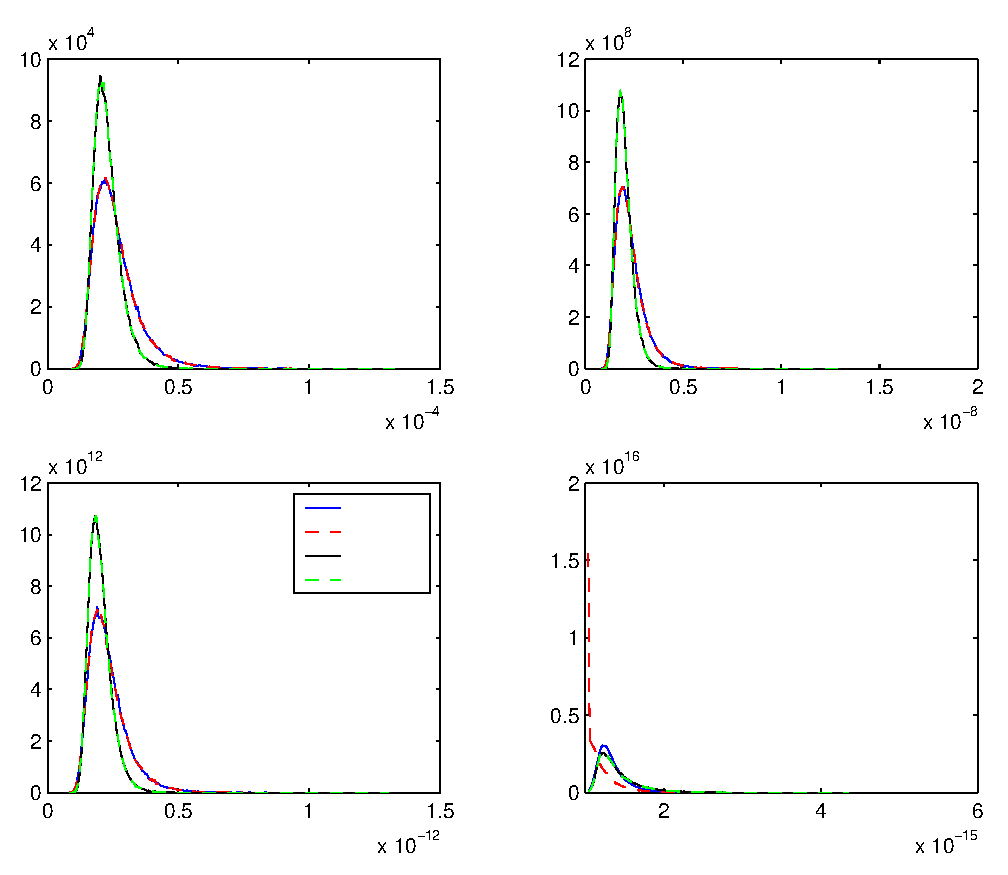
\includegraphics[width=120mm]{Pics/fig_error_distributions_mod.eps}}
%\put(00,78){$p(e_{25})$}
%\put(65,78){$p(e_{50})$}
\put(02,13){\rotatebox{90}{Empirical density}}
%\put(65,26){$p(e_{100})$}
\put(36,55){$e_{25}$}
\put(101,55){$e_{50}$}
\put(36,03){$e_{75}$}
\put(101,03){$e_{100}$}
\put(33,100){$\ell = 25$}
\put(33,48){$\ell = 75$}
\put(98,100){$\ell = 50$}
\put(98,48){$\ell = 100$}
\put(48,42.5){\footnotesize Gauss}
\put(48,39.5){\footnotesize Ortho}
\put(48,36.5){\footnotesize SRFT}
\put(48,33.5){\footnotesize GSRFT}
\end{picture}
\end{center}
\caption{{\rm Empirical probability density functions for the error in Algorithm \ref{alg:basic}.}
As described in~\S\ref{sec:num_SRFT}, the algorithm is implemented with four
distributions for the random test matrix and used to approximate the $200\times 200$ input matrix obtained by
discretizing the integral operator \eqref{eq:int_op_laplace}.
The four panels capture the empirical error distribution for each version of the algorithm
at the moment when $\ell = 25, 50, 75, 100$ random samples have been drawn.}
\label{fig:SRFT_errors}
\end{figure}

%In practice, $\ell = k \log k$ is a reasonable choice for the
%sampling parameter. Although the factor $\log k$ cannot generally be
%removed, experiments suggest that the selection $\ell = k + 20$ is
%often adequate.\footnote{I find the message of this paragraph slightly
%unclear: Are we saying that $\ell = k\log k$ is a good choice, or that
%$\ell = k+20$ is a good choice? Maybe we could write something along
%the lines:

%The likelihood of error with an SRFT test matrix is much higher than
%in the Gaussian case.  In practice, the failure probability here is
%polynomial in $k^{-1}$, while in the Gaussian failure probability is
%$\econst^{-(\ell - k)}$ or better.  This difference is not an
%artifact of the analysis.  Discrete sampling techniques inherently
%fail with higher probability because of the coupon collector's
%problem (Remark~\ref{remark:coupon}). \notate{Fix me.}

%~\cite{Fel68:Introduction-Probability}.
%\pgnotate{Would a reference to Remark \ref{remark:coupon} be in order?}

%\notate{Discussion of what this result means.  We can't leverage
%the detailed error bound because there's no independence between
%$\mtx{\Omega}_1$ and $\mtx{\Omega}_2$ anymore.  In the
%introduction, if we cite a result, it is probably better just to
%replace the numerical constants with letters.  The values here
%really have no significance.}

%\notate{Check probabilities}

We complete the section with the proof of Theorem~\ref{thm:SRFT}.


\input{main82.bbl}

\end{document}
